%% ============================================================================
%% Signal-Adaptive GraphRAG for Traditional Chinese Bible QA — full paper
%% IEEE journal format (IEEEtran). Compile: pdflatex main && pdflatex main
%% (bibliography is a manual thebibliography, ordered by first citation)
%% ============================================================================
\documentclass[journal]{IEEEtran}

\usepackage{cite}
\usepackage{amsmath,amssymb,amsfonts}
\usepackage{graphicx}
\usepackage{booktabs}
\usepackage{multirow}
\usepackage{threeparttable}
\usepackage{algorithm}
\usepackage{algorithmic}
\usepackage{tikz}
\usetikzlibrary{arrows.meta,shapes.geometric,positioning,fit,calc}
\usepackage{pgfplots}
\pgfplotsset{compat=1.18}
\usepackage{balance}
\usepackage[hidelinks]{hyperref}

% ---------------------------------------------------------------------------
% shorthand macros
\usepackage{xspace}
\newcommand{\eg}{e.g.,\xspace}
\newcommand{\fusedeq}{\ensuremath{s_{\mathrm{fused}} = (1-\alpha)\, s_{\mathrm{rr}} + \alpha\, w}\xspace}
\newcommand{\code}[1]{\texttt{\small #1}}

\begin{document}

\title{Signal-Adaptive GraphRAG for Traditional Chinese Bible Question
Answering: End-to-End Architecture, Knowledge-Graph Quality Remediation,
and Rank Fusion}

\author{Ko-Han~Chung, Yoke-Hou~Tan%
\thanks{K.-H. Chung and Y.-H. Tan are with the Department of Intelligent
Computing and Big Data, Chung Yuan Christian University, Taoyuan City,
Taiwan (corresponding author: Y.-H. Tan).}%
\thanks{Manuscript drafted July 7, 2026. All corpus, graph, and evaluation
statistics were re-verified against the live deployment on July 6, 2026.}}

\markboth{Preprint — July 2026}%
{Chung \MakeLowercase{\textit{et al.}}: Signal-Adaptive GraphRAG for Traditional Chinese Bible QA}

\maketitle

\begin{abstract}
Domain-specific question answering (QA) with large language models (LLMs)
faces high API cost, data-privacy constraints, and strict factuality
requirements. We present the complete design, deployment, and three-round
empirical optimization of a graph-based retrieval-augmented generation
(GraphRAG) system for Traditional Chinese Bible QA. The offline pipeline
converts 66 books of the Chinese Union Version from PDF into a
pericope-centric hierarchical corpus by layout-geometry analysis, applies
token-aware hierarchical chunking, and builds a knowledge graph with
grounded dual-track entity extraction (9{,}120 entities of six types;
173{,}896 mentions), closed-schema grounded relation extraction (37
relation types), and a 250{,}418-edge cross-reference network that
integrates the Treasury of Scripture Knowledge. Content, vectors, and graph
are stored in PostgreSQL, Qdrant, and Neo4j, and served online by a
signal-driven six-route retrieval architecture with eleven strategies,
cross-encoder reranking, and a linear rank-fusion layer
$s_{\mathrm{fused}}=(1-\alpha)\,s_{\mathrm{rr}}+\alpha\,w$. On a
100-question benchmark spanning five question types we report a three-round
evidence chain: (i) signal-adaptive retrieval beats a semantic-only
baseline by $+15$ percentage points hit rate, independently of the answer
model; (ii) a knowledge-graph completeness overhaul (entity anchor coverage
$83.8\%\!\rightarrow\!98.2\%$, cross-references $\times 273$) yields
\emph{zero} retrieval gain on the head-entity benchmark --- a negative
result we diagnose, question by question, to a reranker-monopolized final
ranking, topical cross-reference noise, and benchmark head saturation; and
(iii) a one-day rank-fusion remediation recovers and surpasses all prior
results (hit rate $0.97$, event-narrative hit rate $1.00$, $+0.16$ over the
semantic baseline), with an ablation showing a complementary structure
between discrete data repairs and continuous score fusion. We conclude that
knowledge-graph construction quality, the retrieval ranking mechanism, and
benchmark design \emph{jointly} determine observable benefit, and that
optimization order should follow the bottleneck layer rather than the
upstream-first order of the data flow.
\end{abstract}

\begin{IEEEkeywords}
Evaluation methodology, GraphRAG, knowledge graph construction,
negative results, question answering, rank fusion, retrieval-augmented
generation, Traditional Chinese.
\end{IEEEkeywords}

\IEEEpeerreviewmaketitle

%% ============================================================================
%% Section I: Introduction  +  Section II: Related Work
%% ============================================================================

\section{Introduction}
\label{sec:intro}

\IEEEPARstart{L}{arge} language models (LLMs) excel at open-domain question
answering, but deploying them for a specific knowledge domain exposes three
persistent obstacles. First, commercial API pricing places a recurring cost
on every query, which is prohibitive for resource-constrained organizations
such as churches, seminaries, and non-profit publishers. Second, sensitive
corpora and user questions often cannot leave the premises, ruling out
cloud-only inference. Third, and most specific to the religious domain,
factual grounding is non-negotiable: recent measurements report that even
state-of-the-art LLMs score lowest on faith-related dimensions of a
human-flourishing alignment benchmark~\cite{hilliard2025flourishing},
reinforcing a legitimate concern in the Christian community about whether
LLM answers are actually grounded in Scripture rather than in the model's
parametric memory.

Retrieval-augmented generation (RAG)~\cite{lewis2020rag} mitigates factual
errors by conditioning generation on retrieved evidence, and graph-based
RAG (GraphRAG) variants~\cite{edge2024graphrag,peng2026graphragsurvey}
additionally exploit entity and relation structure for multi-hop and
aggregation queries. However, most published GraphRAG systems are evaluated
as end-to-end black boxes: when a knowledge graph (KG) improvement does or
does not move the final metric, the community rarely learns \emph{which
layer} --- extraction, storage, retrieval, ranking, generation, or the
benchmark itself --- gated the outcome. This paper documents a deployed
system in which exactly that question was forced into the open, three
times, by concrete engineering incidents.

We design, build, deploy, and iteratively optimize a GraphRAG system for
question answering over the Traditional Chinese Bible (Chinese Union
Version, new punctuation edition; CUV). The system converts 66 books from
PDF into a pericope-centric hierarchical corpus, constructs a knowledge
graph with grounded entity and relation extraction, indexes three
complementary databases (PostgreSQL, Qdrant, Neo4j), and serves queries
through a signal-driven six-route retrieval architecture terminated by a
cross-encoder reranker and a linear rank-fusion layer. Along the way we
performed a quantified audit of KG construction quality, executed a
completeness overhaul, observed a rigorously verified \emph{negative
result} --- the overhaul produced zero retrieval improvement on our
benchmark --- diagnosed the mechanism question by question, and repaired
the actual bottleneck (the ranking layer) in one day of engineering,
surpassing all previous results.

This paper makes six contributions:

\begin{enumerate}
\item \textbf{A complete, reproducible pipeline from raw PDF to GraphRAG
for Traditional Chinese biblical text} (Sections~\ref{sec:preprocessing}
and~\ref{sec:kg}): layout-geometry PDF parsing without OCR or LLMs,
pericope-centric hierarchical chunking with the embedding model's own
tokenizer, grounded dual-track entity extraction (six types, 9{,}120
entities, 173{,}896 mentions), closed-schema grounded relation extraction
(37 relation types with evidence-span verification), and a three-source
cross-reference network of 250{,}418 edges integrating the public-domain
Treasury of Scripture Knowledge (TSK)~\cite{tsk}.

\item \textbf{A signal-adaptive six-route retrieval architecture over a
triple-database backend, terminated by a rank-fusion layer}
(Section~\ref{sec:retrieval}): six boolean query signals select among six
routes plus a fallback; each route runs a weighted combination of eleven
retrieval strategies; candidates are deduplicated, reranked by a
cross-encoder, fused by
$s_{\mathrm{fused}}=(1-\alpha)\,s_{\mathrm{rr}}+\alpha\,w$, and finally
adjusted by a small set of ``user-literal'' pins.

\item \textbf{A quantified causal chain from chunking granularity to KG
quality} (Section~\ref{sec:audit}): we show that the damage to KG quality
was caused not by chunk-size parameters but by the \emph{silent
inheritance} of an embedding-oriented granularity structure by the
extraction, import, and retrieval layers (mechanisms M1--M6), producing a
55.9\% silent mention loss and 1{,}474 retrieval-blind entities. The
finding is aligned with, and locally re-validates, published evidence on
extraction granularity~\cite{edge2024graphrag}, document-level relation
extraction~\cite{yao2019docred}, and coreference-resolved KG
construction~\cite{meher2025corekg,meher2025insidecorekg,meher2025linkkg}.

\item \textbf{A verified negative result with a mechanism-level diagnosis}
(Section~\ref{sec:p0}): a KG completeness overhaul that raised entity
anchor coverage from 83.8\% to 98.2\% and multiplied cross-references by
273 produced \emph{no} improvement --- and locally a regression --- on a
100-question head-entity benchmark. Question-by-question forensics
attribute this to (a) topical cross-reference votes acting as noise on
event-narrative questions, (b) a final ranking monopolized by the
cross-encoder's surface-form score, and (c) benchmark head saturation. This
result complements benchmark-level observations that KG defects propagate
non-linearly to answers~\cite{zhou2025brink} and that GraphRAG gains are
frequently over-read due to evaluation bias~\cite{zeng2025unbiased}.

\item \textbf{A rank-fusion remediation with an interpretable ablation}
(Section~\ref{sec:fusion}): TSK de-noising by vote-weighted edge
declassing, a curated head-event backfill that re-enabled entity-vector
retrieval, and the linear fusion layer together lift hit rate to 0.97
(event-narrative questions to 1.00), surpassing the pre-overhaul state and
widening the margin over the semantic-only baseline to $+0.16$. The
$\alpha$ ablation exposes a complementary structure --- discrete data
repairs saturate hit rate, continuous fusion recovers tail anchors --- and
a mechanism-level finding that discrete ``pin'' patches flip from
net-positive to net-negative once continuous fusion exists.

\item \textbf{A methodological conclusion for GraphRAG practice}
(Section~\ref{sec:discussion}): KG construction quality, the retrieval
ranking mechanism, and benchmark design jointly determine the observable
benefit of any single-layer investment. In our deployment, one day of
ranking-layer repair outperformed what a week-scale re-extraction was
projected to deliver on the same benchmark; three independent incident
rounds show graph assets whose value was gated by retrieval-side
mechanisms. We argue that evaluation design is a \emph{prerequisite} for
--- not an afterthought of --- further construction-side optimization.
\end{enumerate}

The remainder of the paper follows the pipeline order: corpus and
preprocessing (Section~\ref{sec:preprocessing}), knowledge-graph
construction (Section~\ref{sec:kg}), online retrieval and generation
(Section~\ref{sec:retrieval}), the evaluation framework
(Section~\ref{sec:eval}), the quality audit and the three experiment
rounds (Sections~\ref{sec:round0}--\ref{sec:fusion}), discussion
(Section~\ref{sec:discussion}), limitations and future work
(Sections~\ref{sec:limitations}--\ref{sec:future}), and conclusion
(Section~\ref{sec:conclusion}). Appendix~\ref{app:citations} maps each
pipeline stage to the literature it draws on.

\section{Related Work}
\label{sec:related}

\subsection{Retrieval-Augmented Generation and Hybrid Retrieval}

RAG~\cite{lewis2020rag} couples a parametric generator with non-parametric
retrieval; surveys~\cite{gao2023ragsurvey} catalogue its now-extensive
design space. Dense passage retrieval~\cite{karpukhin2020dpr} and lexical
scoring~\cite{robertson2009bm25} remain the two complementary retrieval
substrates, commonly combined by reciprocal rank fusion
(RRF)~\cite{cormack2009rrf}. Our system uses BGE-M3~\cite{chen2024bgem3}
for dense embeddings (and its companion cross-encoder,
BGE-reranker-v2-m3, for reranking), BM25 with Chinese-specific CKIP
tokenization~\cite{ckip} for sparse vectors, and RRF for dense--sparse
hybrid search. Distinct from standard hybrid search, the final ranking in
our system linearly fuses the cross-encoder score with a
\emph{strategy-prior} weight that encodes which retrieval strategy
proposed the candidate --- a channel by which graph evidence survives into
the final top-$k$ (Section~\ref{sec:fusionlayer}). Calibrated fusion of
heterogeneous graph and vector scores has recently been studied in
multi-hop QA~\cite{bacellar2026calibrated}; our fusion is deliberately
simpler (a single linear interpolation with one global $\alpha$) and is
evaluated by ablation.

\subsection{Graph-Based RAG}

GraphRAG~\cite{edge2024graphrag} popularized LLM-built entity graphs with
hierarchical community summaries for query-focused summarization;
subsequent systems explore lighter indexing and different retrieval
operators, \eg LightRAG's dual-level keyword retrieval~\cite{guo2024lightrag},
personalized-PageRank retrieval over passage-linked
graphs~\cite{gutierrez2025hipporag2}, attributed-community hierarchical
retrieval~\cite{wang2025archrag}, and recursive abstractive summary trees
(RAPTOR)~\cite{sarthi2024raptor}. Event-centric variants build explicit
event nodes and temporal edges~\cite{zhang2025entityevent,sun2025dygrag}.
Benchmark studies ask \emph{when} graphs actually help
RAG~\cite{xiang2025whengraphs}. Our architecture differs from these
retrieval-operator designs in that graph traversal is one of ten
strategies selected \emph{per query} by boolean signals (route-level
adaptivity), and in that the paper's empirical focus is not a new
operator but the interaction between graph asset quality, ranking, and
benchmark --- an interaction that, to our knowledge, has not been
documented at incident-level granularity for a deployed GraphRAG system.

\subsection{LLM-Based Knowledge Graph Construction}

LLM-driven KG construction is surveyed in~\cite{bian2025kgsurvey}, which
contrasts schema-based and schema-free extraction paradigms; our relation
extractor is schema-based with a closed 37-type ontology. On construction
quality, GraphRAG's own ablation shows chunk granularity directly controls
extraction density (600- vs.\ 2{,}400-token chunks yield nearly twice the
entity references)~\cite{edge2024graphrag}; DocRED quantifies that at
least 40.7\% of relational facts require cross-sentence evidence and
17.6\% require coreference reasoning~\cite{yao2019docred}; and
``lost-in-the-middle'' effects bound how much context can be packed into a
single extraction call~\cite{liu2024lost}. Coreference-resolved
construction reduces node duplication by 28--45\% in the CORE-KG /
LINK-KG line of work~\cite{meher2025corekg,meher2025insidecorekg,%
meher2025linkkg}, with the ablation in~\cite{meher2025insidecorekg}
cleanly separating coreference (deduplication) from structured prompting
(noise suppression). Post-extraction correction is an alternative to
re-extraction: ontology-grounded repair~\cite{loconte2026betterlater},
canonicalization after open extraction~\cite{zhang2024edc}, KG denoising
that \emph{shrinks} graphs yet improves downstream RAG~\cite{zheng2025lessismore},
retrieval-augmented construction that re-retrieves cross-chunk context for
each pre-entity~\cite{zhang2025rakg}, restoring the source context of
isolated triples~\cite{huang2025tcrqf}, and GNN-guided cross-chunk graph
augmentation~\cite{zhang2026crossaug}. Atomic-fact decomposition with
dual-time modeling~\cite{lairgi2025atom} shows finer construction units
increase fact coverage. Our audit (Section~\ref{sec:audit}) maps each of
our locally measured defects onto this literature, and our remediation
roadmap adopts its recipes.

\subsection{Evaluating RAG and GraphRAG}

We evaluate generation with RAGAS~\cite{es2023ragas} plus a custom
LLM-judged answer-coverage metric, and retrieval with deterministic
ground-truth metrics. Two recent results shape our methodology. BRINK
benchmarks how KG-based RAG breaks under incomplete knowledge and finds
that answer quality degrades non-linearly with KG defects, with systems
partly relying on parametric memory rather than structural
reasoning~\cite{zhou2025brink}. An unbiased evaluation framework for
GraphRAG shows that after removing position and verbosity bias from
LLM-judged comparisons, reported win rates can drop by tens of points
(\eg LightRAG $66.70\%\!\rightarrow\!39.06\%$)~\cite{zeng2025unbiased}. Our
own evaluation encountered a concrete instance of judge bias --- the RAGAS
answer-relevancy ``noncommittal'' rule zeroes honest refusals, deflating
the score of a cautious commercial model (Section~\ref{sec:evalmetrics}).
Chunking-strategy sensitivity for \emph{retrieval} (not construction) has
been studied systematically in~\cite{shaukat2026chunking}; we cite it only
for its retrieval-side scope, since no peer-reviewed quantification exists
for overlap effects on \emph{extraction}, and we rely on
DocRED~\cite{yao2019docred} as indirect evidence there.

%% ============================================================================
%% Section III: Corpus and Data Preprocessing
%% ============================================================================

\section{Corpus and Data Preprocessing}
\label{sec:preprocessing}

The offline pipeline (Fig.~\ref{fig:offline}) turns 66 books of the CUV
from PDF into (i) a hierarchical structured corpus, (ii) a multi-granular
embedding queue, and (iii) the inputs of knowledge-graph construction. All
build steps run on the host from a dedicated \code{scripts/} environment;
every intermediate artifact is materialized as JSONL before database
import, so each stage is independently inspectable and re-runnable.

\begin{figure*}[!t]
\centering
\resizebox{0.98\textwidth}{!}{%
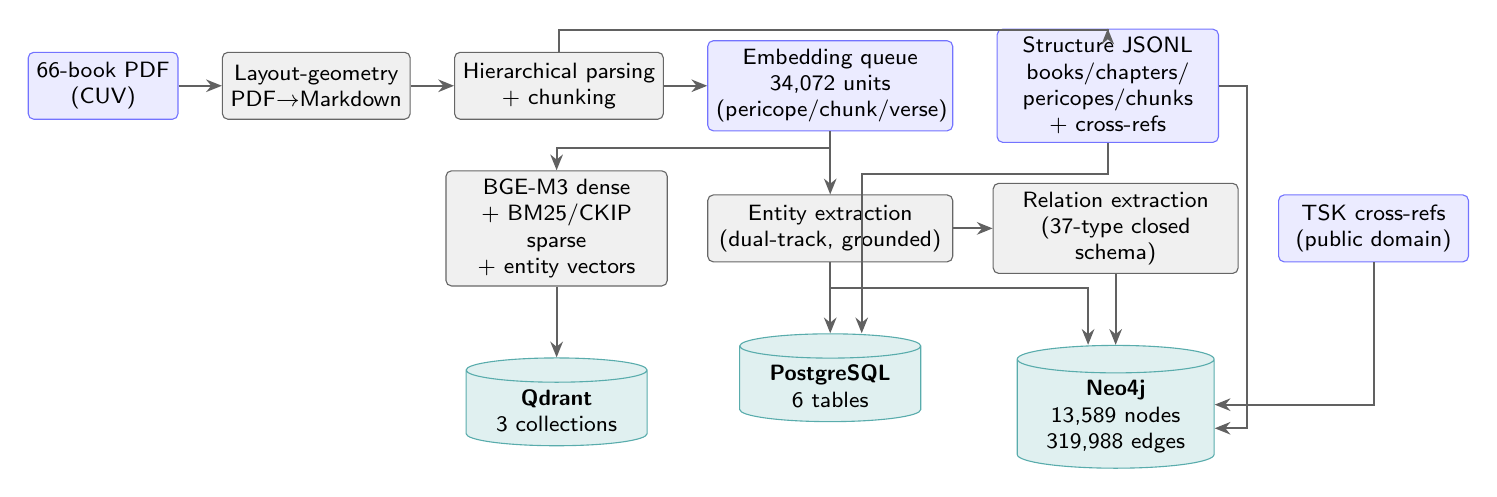
\begin{tikzpicture}[
  font=\sffamily\footnotesize,
  >={Stealth[length=2mm,width=1.6mm]},
  box/.style={rectangle, rounded corners=2pt, draw=black!60, fill=black!6,
              align=center, inner sep=3pt, minimum height=0.85cm},
  data/.style={rectangle, rounded corners=2pt, draw=blue!55, fill=blue!8,
               align=center, inner sep=3pt, minimum height=0.85cm},
  db/.style={cylinder, shape border rotate=90, aspect=0.18, draw=teal!65,
             fill=teal!12, align=center, inner sep=2.5pt},
  flow/.style={->, draw=black!62, line width=0.7pt},
]
% Row 1: source to chunking
\node[data] (pdf) {66-book PDF\\(CUV)};
\node[box, right=0.55cm of pdf] (md) {Layout-geometry\\PDF$\to$Markdown};
\node[box, right=0.55cm of md] (parse) {Hierarchical parsing\\+ chunking};
\node[data, right=0.55cm of parse, text width=2.9cm] (queue)
  {Embedding queue\\34{,}072 units\\(pericope/chunk/verse)};
\node[data, right=0.55cm of queue, text width=2.6cm] (struct)
  {Structure JSONL\\books/chapters/\\pericopes/chunks\\+ cross-refs};

% Row 2: extraction / embedding
\node[box, below=0.8cm of queue.south west, anchor=north west, text width=2.9cm] (ee)
  {Entity extraction\\(dual-track, grounded)};
\node[box, right=0.5cm of ee, text width=2.9cm] (re)
  {Relation extraction\\(37-type closed schema)};
\node[box, left=0.5cm of ee, text width=2.6cm] (emb)
  {BGE-M3 dense\\+ BM25/CKIP sparse\\+ entity vectors};
\node[data, right=0.5cm of re, text width=2.2cm] (tsk)
  {TSK cross-refs\\(public domain)};

% Row 3: databases
\node[db, below=0.9cm of emb, minimum width=2.3cm, minimum height=1.05cm] (qd)
  {\textbf{Qdrant}\\3 collections};
\node[db, below=0.9cm of ee, minimum width=2.3cm, minimum height=1.05cm] (pg)
  {\textbf{PostgreSQL}\\6 tables};
\node[db, below=0.9cm of re, minimum width=2.5cm, minimum height=1.05cm] (neo)
  {\textbf{Neo4j}\\13{,}589 nodes\\319{,}988 edges};

\draw[flow] (pdf) -- (md);
\draw[flow] (md) -- (parse);
\draw[flow] (parse) -- (queue);
\draw[flow] (parse.north) -- ++(0,0.28) -| (struct.north);
\draw[flow] (queue.south) |- ($(ee.north)+(0,0.28)$) -- (ee.north);
\draw[flow] (queue.south) |- ($(emb.north)+(0,0.28)$) -- (emb.north);
\draw[flow] (ee) -- (re);
\draw[flow] (emb) -- (qd);
\draw[flow] (ee) -- (pg);
\draw[flow] (re) -- (neo);
\draw[flow] (tsk.south) |- ($(neo.east)+(0.25,0.15)$) -- ($(neo.east)+(0,0.15)$);
\draw[flow] (struct.east) -| ++(0.35,-3.1) |- ($(neo.east)+(0,-0.15)$);
\draw[flow] (ee.south) -- ++(0,-0.33) -| ($(neo.north)+(-0.35,0)$);
\draw[flow] (struct.south) -- ++(0,-0.4) -| ($(pg.north)+(0.4,0)$);
\end{tikzpicture}%
}
\caption{Offline build pipeline. Every arrow is a materialized JSONL
hand-off; the three databases play complementary roles
(Section~\ref{sec:tripledb}); database counts show the live
post-remediation state (July 6, 2026). The embedding queue doubles as
the extraction feed --- the structural root cause analyzed in
Section~\ref{sec:audit} (mechanism M1).}
\label{fig:offline}
\end{figure*}

\subsection{Source Corpus}

The source is the Chinese Union Version with new punctuation, obtained as
66 per-book PDFs (one per biblical book). The CUV is the de facto standard
Protestant translation in the Traditional Chinese world; its vocabulary is
early-20th-century literary Chinese, which creates a systematic lexical
gap between modern user phrasing and corpus surface forms --- a gap that
recurs throughout this paper (\eg the modern phrase ``the Last Supper''
never occurs in the CUV text, which narrates a ``Passover meal'').

\subsection{PDF-to-Markdown by Layout Geometry}

Conversion (\code{convert\_bible\_pdf.py}, PyMuPDF) uses \emph{pure layout
geometry} over character-level spans --- no OCR and no LLM --- so the step
is deterministic, free, and auditable:

\begin{itemize}
\item font size $\le 8.5$\,pt: running headers/footers, dropped;
\item font size $\ge 16$\,pt: book title or chapter number;
\item font size $=12$\,pt with $x \ge 85$: pericope (section) heading;
\item font size $\le 9.5$\,pt and numeric: verse number;
\item verse number at $x < 75$ with line right-edge $< 300$: poetry
      (line breaks preserved); otherwise prose (lines joined);
\item bold \code{N:N} tokens: footnotes, aggregated per chapter.
\end{itemize}

The resulting Markdown uses \code{\#} for book, \code{\#\#} for chapter,
\code{\#\#\#} for pericope headings, and bold verse numbers. Under each
pericope heading, the CUV's printed parallel-passage annotations (\eg
``(Mark 1:9--11; Luke 3:21--22)'' under the baptism pericope) are retained
--- they become the first source of the cross-reference network
(Section~\ref{sec:crossrefs}).

\subsection{Pericope-Centric Hierarchical Structure}
\label{sec:pericope}

A \emph{pericope} is the established interpretive unit of biblical
scholarship: a self-contained narrative episode, discourse, or psalm. The
CUV's editorial pericope headings give us this segmentation for free, and
the system adopts the pericope as the core unit for embedding, entity
anchoring, and cross-referencing, for three reasons:

\begin{enumerate}
\item \textbf{Semantic completeness.} A story is never split down the
middle; retrieval returns interpretable wholes.
\item \textbf{Embedding fit.} The median pericope is 388 characters
(P90 $=931$, max $=3{,}544$), well inside the effective input range of the
BGE-M3 embedder~\cite{chen2024bgem3}.
\item \textbf{Explainability.} Returning ``Isaac takes a wife
(Gen.~24)'' is more interpretable to end users than a verse-range span.
\end{enumerate}

Parsing (\code{process\_bible.py} with \code{markdown\_parser.py}) yields
the hierarchy Book\,$\rightarrow$\,Chapter\,$\rightarrow$\,Pericope with
counts 66\,/\,1{,}189\,/\,2{,}779, plus per-pericope verse spans. A
regex-based reference parser with a Chinese book-abbreviation table
resolves the parallel-passage annotations; every reference is
\emph{upgraded to pericope level} (never verse level), keeping the
cross-reference network aligned with the retrieval unit. Hierarchical IDs
are colon-delimited (\code{gen} $\rightarrow$ \code{gen:1} $\rightarrow$
\code{gen:1:0} for the first pericope of Genesis~1), a scheme reused
verbatim across all three databases.

\subsection{Hierarchical Chunking}
\label{sec:chunking}

Long pericopes are split for embedding by a token-aware hierarchical
chunker whose tokenizer is \emph{BGE-M3's own}, i.e., the chunking layer
is explicitly designed for the embedding model~\cite{chen2024bgem3}:

\begin{itemize}
\item pericopes with $\le 768$ tokens (93.9\%) are kept whole;
\item longer pericopes are split on \emph{verse boundaries} targeting 512
tokens per chunk, with a 1-verse overlap between adjacent chunks;
\item a trailing chunk under 128 tokens and $\le 3$ verses is merged back
into its predecessor;
\item chunk IDs extend the parent ID (\code{gen:1:0:0}), preserving the
hierarchy.
\end{itemize}

Only 169 of 2{,}779 pericopes (6.1\%) are split, producing 431 chunks; the
split pericopes concentrate in Old Testament narrative books (Leviticus
13, Judges 12, 1~Samuel 12, Genesis 11, Numbers 11, Joshua 10, Deuteronomy
9, 2~Samuel 9) and account for 18.3\% of the corpus text (243{,}773 of
1{,}329{,}046 characters); their median length is 1{,}353 characters
(max 3{,}544), against a chunk median of 644 (max 796). Each retrieval
unit's embedded text carries a locating prefix ---
``\emph{Book, Chapter $N$, pericope title (verses $X$--$Y$):}'' --- so
vectors encode provenance context. Table~\ref{tab:corpus} summarizes the
corpus.

\begin{table}[!t]
\caption{Corpus and Chunking Statistics (CUV, New Punctuation)}
\label{tab:corpus}
\centering
\begin{tabular}{lr}
\toprule
Item & Value \\
\midrule
Books & 66 \\
Chapters & 1{,}189 \\
Pericopes & 2{,}779 \\
\quad -- split into chunks & 169 (6.1\%) \\
Chunks (from split pericopes) & 431 \\
Corpus size (characters) & 1{,}329{,}046 \\
\quad -- inside split pericopes & 243{,}773 (18.3\%) \\
Pericope length, median / P90 / max (chars) & 388 / 931 / 3{,}544 \\
Split-pericope length, median / max (chars) & 1{,}353 / 3{,}544 \\
Chunk length, median / max (chars) & 644 / 796 \\
\midrule
Chunker: split threshold / target / min (tokens) & 768 / 512 / 128 \\
Chunker: overlap & 1 verse \\
Tokenizer & BGE-M3 \\
\bottomrule
\end{tabular}
\end{table}

\subsection{Multi-Granularity Embedding Queue}
\label{sec:queue}

Retrieval needs different granularities for different question shapes, so
the pipeline emits an embedding queue that is the union of three levels,
34{,}072 units in total:

\begin{itemize}
\item \textbf{pericope level} (2{,}610): every pericope that was
\emph{not} split;
\item \textbf{chunk level} (431): split pericopes enter only as chunks;
\item \textbf{verse level} (31{,}031): every verse individually, for
fine-grained exact retrieval (printed verse ranges such as ``1--2'' are
kept as single units).
\end{itemize}

This queue is an artifact designed \emph{for retrieval}. Critically for
what follows, the early entity-extraction pipeline consumed this same
queue as its input feed. That single wiring decision --- extraction feed
$=$ embedding queue --- silently propagated an embedding-oriented
granularity into the knowledge graph and became the structural root cause
(M1) of the defect chain quantified in Section~\ref{sec:audit}.

%% ============================================================================
%% Section IV: Knowledge Graph Construction
%% ============================================================================

\section{Knowledge Graph Construction}
\label{sec:kg}

The knowledge graph comprises three subnetworks --- the corpus hierarchy,
the entity network, and the cross-reference network --- built by the four
pipelines described below. Throughout construction we enforce a single
anti-hallucination discipline, \emph{grounding}: LLMs never invent
entities, relation types, or evidence; they only \emph{classify}
candidates that rule-based stages propose, and every LLM output must quote
an evidence span that is verified post hoc to be a literal substring of
the source text, otherwise the output is demoted or discarded. This is the
schema-based end of the paradigm spectrum surveyed
in~\cite{bian2025kgsurvey}, and the structured-prompting choice follows
the noise-suppression evidence of~\cite{meher2025corekg,meher2025insidecorekg}.

\subsection{Grounded Dual-Track Entity Extraction}
\label{sec:entity}

Entity extraction targets six types (Table~\ref{tab:entities}) and runs
two tracks in parallel: a named-entity-recognition (NER) track and a
grounded classification track.

\begin{table}[!t]
\caption{Entity Types (Live Graph Counts, July 6, 2026)}
\label{tab:entities}
\centering
\begin{threeparttable}
\begin{tabular}{llr}
\toprule
Type & Examples & Count \\
\midrule
Person & Abraham, Moses, Jesus & 2{,}419 \\
Object & Ark of the Covenant, tabernacle & 2{,}200 \\
Event  & the Exodus, the Resurrection & 1{,}714 \\
Place  & Jerusalem, Egypt & 1{,}299 \\
Theme  & redemption, grace, faith & 987 \\
Group  & Israelites, Pharisees & 505 \\
\midrule
Total  & & 9{,}124 \\
\bottomrule
\end{tabular}
\begin{tablenotes}\footnotesize
\item Live counts differ slightly from the raw extraction output
(9{,}120; Section~\ref{sec:entity}) because of import-time merging and
the post-audit curation of Sections~\ref{sec:p0}--\ref{sec:fusion}
(16 generic-noun events deleted, 18 curated events added, one entity
retyped); the pre-remediation live count, used by the audit of
Section~\ref{sec:audit}, was 9{,}122.
\end{tablenotes}
\end{threeparttable}
\end{table}

\subsubsection{NER Track (Person / Place / Group)}
CKIP Transformers~\cite{ckip} performs Chinese word segmentation and named
entity recognition (BERT-base models), with the type mapping
PERSON$\to$Person, GPE/LOC$\to$Place, ORG/NORP$\to$Group. Results are
merged with a hand-built biblical entity dictionary using
dictionary-first, longest-match precedence. Mention positions are located
by literal string matching (\code{text.find()}) --- a design whose
consequences (no coreference; substring false hits) are quantified in
Section~\ref{sec:audit}.

\subsubsection{Grounded Track (Event / Object / Theme)}
Four phases, rule-first with LLM escalation:

\begin{enumerate}
\item \textbf{Pericope-title mining.} Titles are typed by suffix and
keyword heuristics (altar/vessel/ark suffixes $\to$ Object;
redemption/grace keywords $\to$ Theme; residual default $\to$ Event). A
24-word generic-title stoplist (``day(s)'', ``firstborn'', \ldots)
intercepts generic nouns before the Event default --- a guard added after
the noise audit of Section~\ref{sec:audit}.
\item \textbf{POS candidate mining.} CKIP part-of-speech tagging proposes
nouns (Na/Nb/Nv/Nc) with corpus frequency $\ge 3$; adjacent nouns are
compounded (\eg ``burnt'' $+$ ``offering'').
\item \textbf{Rule classifier.} Exact lexicons and verb-component
features assign types; candidates with confidence $\ge 0.8$ are finalized
without any LLM call.
\item \textbf{LLM classifier (grounded).} Remaining candidates are
classified by a small local model (Gemma~3
4B~\cite{gemmateam2025gemma3}) under two hard constraints: it may only
label \emph{provided} candidates (never add new ones), and it must return
an evidence quotation that post-hoc verification confirms is a substring
of the grounding text; failures are demoted.
\end{enumerate}

An \code{EntityNormalizer} merges canonical names and aliases within each
type and assigns \code{entity\_id} $=$ \code{\{type\}:\{pinyin\}}
(toneless \code{lazy\_pinyin} --- a homophone-collision risk noted in
Section~\ref{sec:limitations}). The extraction output is 9{,}120 entities
and 173{,}896 mentions; mentions carry the granularity of their source
unit (pericope, chunk, or verse), inherited from the embedding queue
(Section~\ref{sec:queue}). Known upstream limitations, all revisited in
the audit: a stopword list removes 33 single-character words including
``God'', ``Spirit'', and ``Lord''; there is no coreference resolution;
entity descriptions are 100-character text snippets; and pinyin IDs can
collide across homophones.

\subsection{Grounded Relation Extraction with a Closed 37-Type Ontology}
\label{sec:relation}

Entity--entity fact edges are extracted by a five-stage pipeline against a
closed ontology of 37 relation types (Table~\ref{tab:ontology}), each
declaring domain/range types, direction, inverse, textual trigger
signals, few-shot examples, and per-stage confidence priors. Closing the
schema prevents the LLM from inventing relation names, and typing the
domain/range prunes the candidate space before any model call.

\begin{table}[!t]
\caption{Closed Relation Ontology (37 Types)}
\label{tab:ontology}
\centering
\begin{threeparttable}
\begin{tabular}{p{2.35cm}p{5.6cm}}
\toprule
Type pair (count) & Relations \\
\midrule
Person$\times$Person (13) & \textsc{father\_of, mother\_of, son\_of,
daughter\_of, sibling\_of, spouse\_of, ancestor\_of, descendant\_of,
teacher\_of, disciple\_of, enemy\_of, ally\_of, succeeded\_by} \\
Person$\times$Place (7) & \textsc{born\_in, died\_in, ruled, visited,
exiled\_to, returned\_from, built} \\
Person$\times$Object (4) & \textsc{possessed, received, gave, destroyed} \\
Person$\times$Event (3) & \textsc{participated\_in, initiated,
victim\_of} \\
Person$\times$Group (3) & \textsc{member\_of, leader\_of, founded} \\
Place$\times$Place (2) & \textsc{located\_in, near} \\
Event$\times$Place (1) & \textsc{occurred\_in} \\
Event$\times$Event (2) & \textsc{preceded\_by, caused} \\
Group$\times$Place (2) & \textsc{originated\_from, settled\_in} \\
\bottomrule
\end{tabular}
\begin{tablenotes}\footnotesize
\item Each type defines domain/range, direction, inverse type, regex
trigger signals, few-shot examples, and stage-specific confidence priors.
\end{tablenotes}
\end{threeparttable}
\end{table}

\begin{enumerate}
\item \textbf{Pair mining.} Entity pairs co-occurring in the same
pericope are enumerated, kept only if some ontology type admits their
type signature, and capped at 80 pairs per pericope.
\item \textbf{Rule classifier.} Per-type regex trigger signals fire when
the two entities are within 25 characters; matches with confidence
$\ge 0.85$ are finalized.
\item \textbf{Domain priors.} 71 curated golden genealogy relations
bypass the LLM entirely (64 of them enter the graph as distinct
prior-stage edges; the remainder coincide with earlier-stage matches).
\item \textbf{Grounded LLM classification.} A local Gemma~4 31B
model~\cite{gemma4} --- the relation stage was built after the entity
stage and uses a larger model; the entity classifier's 4B scale is
itself flagged in the audit --- must select exactly one type from the
pair's type-legal candidate set \emph{or} answer \textsc{none}, under a
JSON grammar constraint; the
returned \code{evidence\_span} must pass substring verification against
the source pericope (doubly checked post hoc), otherwise the pair is
rejected. This addresses the classic failure mode of triples divorced
from their source context~\cite{huang2025tcrqf}.
\item \textbf{Inverse materialization.} Symmetric/inverse types
(\textsc{father\_of}\,$\leftrightarrow$\,\textsc{son\_of}) are
materialized bidirectionally at confidence $\times 0.9$.
\end{enumerate}

The full run (10--20 hours offline, checkpointed and resumable) yields
6{,}958 imported relations (772 rule, 64 prior, 5{,}370 LLM, 752 inverse)
--- and, importantly, 77{,}953 \emph{unclassified} candidate pairs
(LLM answered \textsc{none}) retained on disk with their source-pericope
provenance. This ``rejected pile'' later became the raw material of the
P0 event-layer rescue (Section~\ref{sec:p0}). A companion description
generator (Gemma~4 E4B) targets the $\sim$4{,}223 Person/Place/Group
entities with empty descriptions, generating $\le 80$-character
summaries grounded in the titles of mentioning pericopes; entities
without pericope anchors cannot be described this way --- which is why
the audit of Section~\ref{sec:audit} still finds 46\% of NER-type
entities description-less.

Every fact edge carries \code{confidence}, \code{evidence\_span},
\code{source\_pericope\_id}, and \code{extraction\_phase}, so all graph
facts are source-traceable and confidence-filterable --- the property
that later allowed co-occurrence backfill edges (confidence 0.35) to
coexist distinguishably with LLM-extracted edges.

\subsection{Cross-Reference Network}
\label{sec:crossrefs}

Cross-references (``chain references'') connect pericopes across books
--- prophecy and fulfillment, parallel gospel accounts, quotations. The
network merges three sources of decreasing editorial cost:

\begin{enumerate}
\item \textbf{Printed parallel-passage annotations} parsed from the CUV
Markdown: 774 edges (synoptic parallels and psalm titles);
\item \textbf{A curated list of famous New-Testament-to-Old-Testament
(NT$\to$OT) citations}: 142 edges typed as \emph{quotation} or
\emph{allusion};
\item \textbf{The Treasury of Scripture Knowledge (TSK)}~\cite{tsk}, a
public-domain cross-reference compendium with community vote counts:
344{,}799 raw rows are filtered (1{,}166 negative-vote rows, 9{,}811
self-loops) and mapped verse$\to$pericope through a reverse index built
from the embedding queue (covering 31{,}102 verses, with printed verse
ranges expanded); only 7 rows fail to map, yielding 250{,}358 unique
pericope pairs.
\end{enumerate}

After idempotent merge the live graph holds \textbf{250{,}418}
\textsc{cross\_references} edges. Every TSK edge stores its \code{votes};
manual edges are assigned a sentinel vote of 999 (highest trust). This
vote-based provenance is what later made \emph{selective de-noising}
possible without deleting data (Section~\ref{sec:fusion}) --- the same
``repair by re-weighting, not removal'' philosophy advocated for KG
denoising in~\cite{zheng2025lessismore}.

\subsection{Graph Schema and Storage}
\label{sec:schema}

\begin{figure}[!t]
\centering
\resizebox{\columnwidth}{!}{%
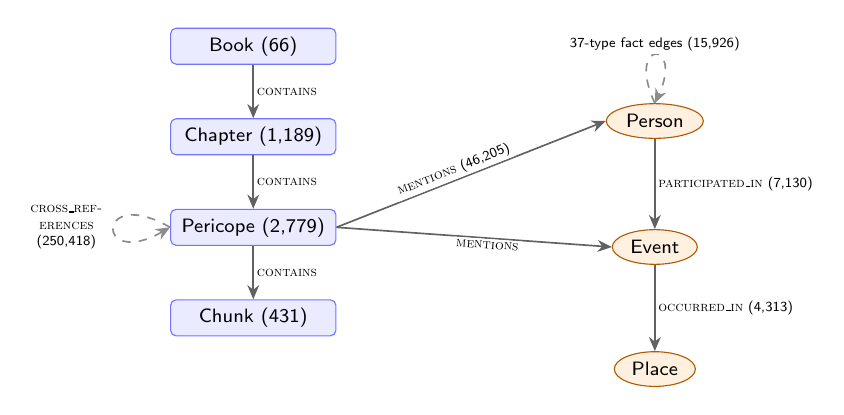
\begin{tikzpicture}[
  font=\sffamily\scriptsize,
  >={Stealth[length=1.8mm,width=1.5mm]},
  hier/.style={rectangle, rounded corners=2pt, draw=blue!55, fill=blue!8,
               align=center, inner sep=3pt, minimum width=2.1cm},
  ent/.style={ellipse, draw=orange!70!black, fill=orange!12,
              align=center, inner sep=2pt},
  edge/.style={->, draw=black!62, line width=0.6pt},
  dedge/.style={->, draw=black!45, line width=0.6pt, dashed},
  elbl/.style={font=\tiny\sffamily, fill=white, inner sep=1pt},
]
\node[hier] (book) at (0,4.7) {Book (66)};
\node[hier] (ch)   at (0,3.55) {Chapter (1{,}189)};
\node[hier] (per)  at (0,2.4) {Pericope (2{,}779)};
\node[hier] (chk)  at (0,1.25) {Chunk (431)};

\node[ent] (person) at (5.1,3.75) {Person};
\node[ent] (event)  at (5.1,2.15) {Event};
\node[ent] (place)  at (5.1,0.6)  {Place};

\draw[edge] (book) -- node[elbl,right]{\textsc{contains}} (ch);
\draw[edge] (ch) -- node[elbl,right]{\textsc{contains}} (per);
\draw[edge] (per) -- node[elbl,right]{\textsc{contains}} (chk);

\draw[edge] (per.east) -- node[elbl,above,sloped,pos=0.45]
  {\textsc{mentions} (46{,}205)} (person.west);
\draw[edge] (per.east) -- node[elbl,below,sloped,pos=0.55]
  {\textsc{mentions}} (event.west);
\draw[edge] (person) -- node[elbl,right]
  {\textsc{participated\_in} (7{,}130)} (event);
\draw[edge] (event) -- node[elbl,right]
  {\textsc{occurred\_in} (4{,}313)} (place);

\draw[dedge] (person.north) to[out=115,in=65,looseness=5,
  min distance=9mm] node[elbl,above]
  {37-type fact edges (15{,}926)} (person.north);

\draw[dedge] (per.west) to[out=150,in=210,looseness=5,
  min distance=11mm] node[elbl,left,align=center,xshift=-1mm]
  {\textsc{cross\_ref-}\\ \textsc{erences}\\(250{,}418)} (per.west);
\end{tikzpicture}%
}
\caption{Knowledge-graph schema: corpus hierarchy (left), entity network
(right), the pericope-to-pericope cross-reference network (774 markdown
$+$ 142 curated $+$ TSK edges), and sequential \textsc{next} /
\textsc{next\_book} edges (omitted for clarity). Verse-level nodes
deliberately do not exist --- the design trade-off whose downstream cost
is quantified in Section~\ref{sec:audit}.}
\label{fig:schema}
\end{figure}

Figure~\ref{fig:schema} shows the schema; Table~\ref{tab:kgscale} the live
scale. Salient design points:

\begin{itemize}
\item \textbf{Dual labels.} Hierarchy nodes carry
\code{(:Pericope:Bible)}, entity nodes \code{(:Person:Entity)}: the
generic label supports whole-structure queries, the specific label exact
matches.
\item \textbf{No verse nodes.} Verse-level IDs (\code{gen:1:0:v:3}) exist
only in Qdrant and PostgreSQL. This was a deliberate economy at design
time --- and the direct precondition of the silent mention-loss defect
(Section~\ref{sec:audit}, M2).
\item \textbf{Entity properties.} \code{canonical\_name},
\code{aliases} (a native list), \code{description}, \code{mention\_count}.
\item \textbf{Provenance-first edges.} Fact edges keep confidence and
evidence; cross-reference edges keep votes and source; backfilled edges
are flagged --- all imports are idempotent \textsc{merge} operations, so
the graph can be rebuilt or rolled back deterministically.
\end{itemize}

\begin{table}[!t]
\caption{Live Knowledge-Graph Scale (Neo4j, July 6, 2026)}
\label{tab:kgscale}
\centering
\begin{tabular}{lr}
\toprule
Item & Count \\
\midrule
Nodes, total & 13{,}589 \\
\quad structure (Book/Chapter/Pericope/Chunk) & 4{,}465 \\
\quad entities (six types) & 9{,}124 \\
Relationships, total & 319{,}988 \\
\quad \textsc{mentions} & 46{,}205 \\
\quad \textsc{cross\_references} & 250{,}418 \\
\quad semantic fact edges (37 types) & 15{,}926 \\
\qquad \textsc{participated\_in} / \textsc{occurred\_in} & 7{,}130 / 4{,}313 \\
\qquad \textsc{son\_of} / \textsc{father\_of} / \textsc{possessed} & 659 / 647 / 551 \\
\quad structural: \textsc{contains} / \textsc{next} / \textsc{next\_book} & 4{,}399 / 2{,}975 / 65 \\
\bottomrule
\end{tabular}
\end{table}

\subsection{Vector Indexes and Database Import}
\label{sec:vectors}

Three vector families are produced:

\begin{itemize}
\item \textbf{Dense}: BGE-M3~\cite{chen2024bgem3}, 1{,}024-dimensional,
normalized, for all 34{,}072 queue units;
\item \textbf{Sparse}: BM25~\cite{robertson2009bm25} ($k_1{=}1.5$,
$b{=}0.75$) over CKIP-segmented~\cite{ckip} text, with the query-side IDF
vocabulary exported for the online service;
\item \textbf{Entity vectors}: each entity is embedded from the recipe
``\emph{name (aliases). description. commonly appears in: pericope
titles}'' truncated to 200 characters, upserted idempotently (UUID5 keys)
into a dedicated collection (9{,}122 points).
\end{itemize}

Imports populate PostgreSQL (6 tables; the authoritative store),
Qdrant (\code{bible\_embeddings}, dense-only;
\code{bible\_embeddings\_hybrid} with named dense$+$sparse vectors;
\code{bible\_entities}), and Neo4j (structure, mentions, fact edges,
cross-references). The import layer is where the audit later found the
single most damaging defect of the whole pipeline --- verse-level
mentions silently dropped because their target nodes do not exist
(Section~\ref{sec:audit}) --- and where honesty counters were
subsequently installed.

%% ============================================================================
%% Section V: Online Retrieval Architecture
%% ============================================================================

\section{Online Retrieval Architecture}
\label{sec:retrieval}

The online service is a FastAPI application exposing
\code{POST /api/v1/query}. Figure~\ref{fig:online} shows the query
pipeline; this section walks through it stage by stage.

\begin{figure*}[!t]
\centering
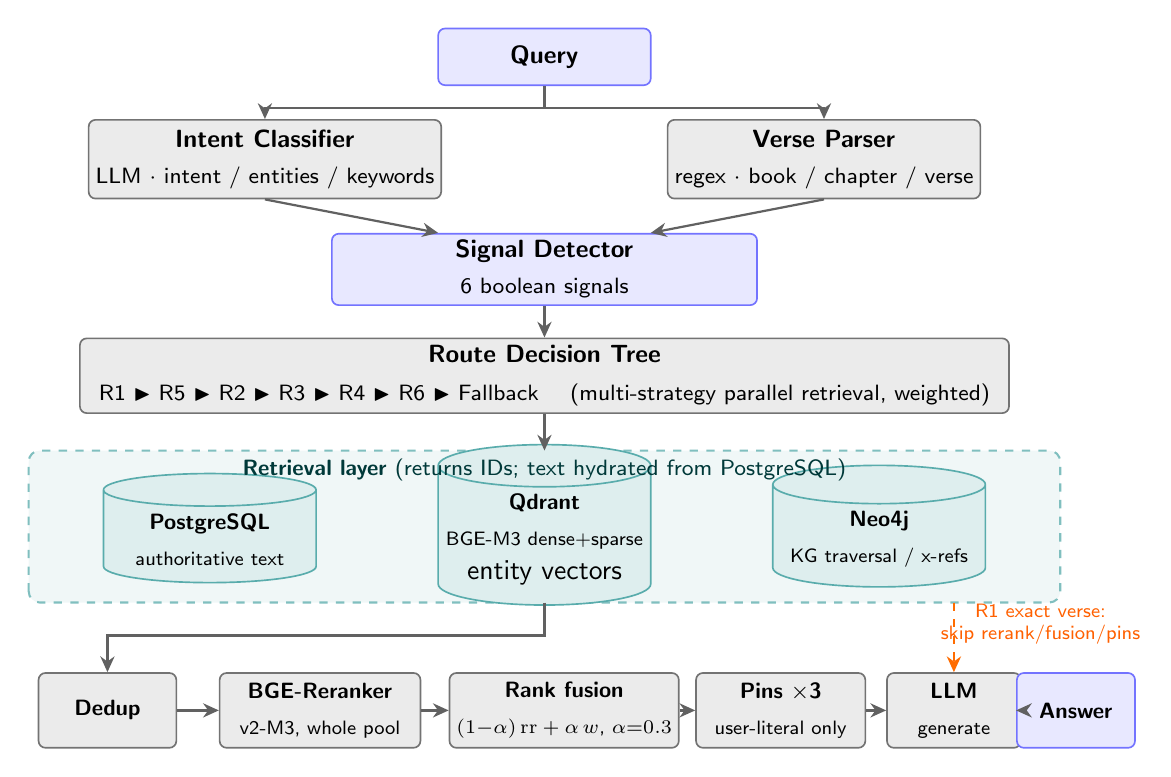
\begin{tikzpicture}[
  font=\sffamily,
  >={Stealth[length=2.0mm,width=1.8mm]},
  stage/.style={rectangle, rounded corners=2.5pt, draw=blue!55, fill=blue!9,
                line width=0.6pt, align=center, inner sep=2.5pt},
  proc/.style={rectangle, rounded corners=2.5pt, draw=black!55, fill=black!8,
               line width=0.6pt, align=center, inner sep=2.5pt},
  db/.style={cylinder, shape border rotate=90, aspect=0.20, draw=teal!65,
             fill=teal!13, line width=0.6pt, align=center, inner sep=2.5pt},
  flow/.style={->, draw=black!62, line width=0.8pt},
  bypass/.style={->, draw=orange!85!red, line width=0.8pt, dashed},
  lbl/.style={font=\scriptsize\sffamily, inner sep=1pt},
]
% Band 1 -- Query
\node[stage, minimum width=2.7cm, minimum height=0.72cm] (query)
  at (7.6,9.55) {\small\textbf{Query}};
% Band 2 -- Intent Classifier | Verse Parser
\node[proc, minimum width=3.7cm, minimum height=1.0cm] (intent) at (4.05,8.25)
  {\small\textbf{Intent Classifier}\\[1pt]
   {\footnotesize LLM $\cdot$ intent / entities / keywords}};
\node[proc, minimum width=3.7cm, minimum height=1.0cm] (vparser) at (11.15,8.25)
  {\small\textbf{Verse Parser}\\[1pt]
   {\footnotesize regex $\cdot$ book / chapter / verse}};
% Band 3 -- Signal Detector
\node[stage, minimum width=5.4cm, minimum height=0.9cm] (signal) at (7.6,6.85)
  {\small\textbf{Signal Detector}\\[1pt]{\footnotesize 6 boolean signals}};
% Band 4 -- Decision tree
\node[proc, minimum width=11.8cm, minimum height=0.95cm] (decision) at (7.6,5.5)
  {\small\textbf{Route Decision Tree}\\[1.5pt]
   {\footnotesize R1 $\blacktriangleright$ R5 $\blacktriangleright$ R2
    $\blacktriangleright$ R3 $\blacktriangleright$ R4 $\blacktriangleright$
    R6 $\blacktriangleright$ Fallback \quad (multi-strategy parallel
    retrieval, weighted)}};
% Band 5 -- Retrieval layer
\draw[draw=teal!50, dashed, line width=0.75pt, rounded corners=4pt,
      fill=teal!6] (1.05,2.62) rectangle (14.15,4.55);
\node[db, minimum width=2.7cm, minimum height=1.15cm] (pg) at (3.35,3.42)
  {\footnotesize\textbf{PostgreSQL}\\[1pt]{\scriptsize authoritative text}};
\node[db, minimum width=2.7cm, minimum height=1.15cm] (qd) at (7.6,3.42)
  {\footnotesize\textbf{Qdrant}\\[1pt]\scriptsize BGE-M3 dense+sparse\\entity vectors};
\node[db, minimum width=2.7cm, minimum height=1.15cm] (n4) at (11.85,3.42)
  {\footnotesize\textbf{Neo4j}\\[1pt]{\scriptsize KG traversal / x-refs}};
\node[font=\footnotesize\sffamily, text=teal!45!black] at (7.6,4.3)
  {\textbf{Retrieval layer} (returns IDs; text hydrated from PostgreSQL)};
% Band 6 -- post-retrieval chain
\node[proc, minimum width=1.75cm, minimum height=0.95cm] (dedup) at (2.05,1.25)
  {\footnotesize\textbf{Dedup}};
\node[proc, minimum width=2.55cm, minimum height=0.95cm] (rerank) at (4.75,1.25)
  {\footnotesize\textbf{BGE-Reranker}\\[1pt]{\scriptsize v2-M3, whole pool}};
\node[proc, minimum width=2.75cm, minimum height=0.95cm] (fuse) at (7.85,1.25)
  {\footnotesize\textbf{Rank fusion}\\[1pt]
   {\scriptsize $(1{-}\alpha)\,\mathrm{rr}+\alpha\,w$, $\alpha{=}0.3$}};
\node[proc, minimum width=2.15cm, minimum height=0.95cm] (pin) at (10.6,1.25)
  {\footnotesize\textbf{Pins $\times$3}\\[1pt]{\scriptsize user-literal only}};
\node[proc, minimum width=1.7cm, minimum height=0.95cm] (llm) at (12.8,1.25)
  {\footnotesize\textbf{LLM}\\[1pt]{\scriptsize generate}};
\node[stage, minimum width=1.5cm, minimum height=0.95cm] (ans) at (14.35,1.25)
  {\footnotesize\textbf{Answer}};
% edges
\draw[flow] (query.south) -- ++(0,-0.28) -| (intent.north);
\draw[flow] (query.south) -- ++(0,-0.28) -| (vparser.north);
\draw[flow] (intent.south) -- ([xshift=-1.35cm]signal.north);
\draw[flow] (vparser.south) -- ([xshift=1.35cm]signal.north);
\draw[flow] (signal.south) -- (decision.north);
\draw[flow] (decision.south) -- (7.6,4.55);
\draw[flow] (7.6,2.62) -- ++(0,-0.42) -| (dedup.north);
\draw[flow] (dedup.east) -- (rerank.west);
\draw[flow] (rerank.east) -- (fuse.west);
\draw[flow] (fuse.east) -- (pin.west);
\draw[flow] (pin.east) -- (llm.west);
\draw[flow] (llm.east) -- (ans.west);
% R1 bypass
\draw[bypass] (12.8,2.62) -- (llm.north);
\node[lbl, text=orange!75!red, align=center] at (13.9,2.35)
  {R1 exact verse:\\skip rerank/fusion/pins};
\end{tikzpicture}
\caption{Online query pipeline. Compared with the May 2026 deployment, the
post-retrieval chain gained the rank-fusion stage, and the pin set was
re-audited: only ``user-literal'' pins survive
(Section~\ref{sec:fusionlayer}).}
\label{fig:online}
\end{figure*}

\subsection{Triple-Database Roles and Content Hydration}
\label{sec:tripledb}

The three stores play strictly complementary roles:

\begin{itemize}
\item \textbf{PostgreSQL} is the authoritative source of truth: full
text, hierarchy, entity mentions. \emph{Every} retrieval strategy returns
only IDs; final passage text is always hydrated by a single PostgreSQL
lookup (\code{get\_content\_by\_id()}), which resolves 3-segment IDs to
pericopes, 4-segment IDs to chunks, and verse IDs to their parent
pericope. This guarantees that no matter which index proposed a
candidate, the generator always sees identical, authoritative text.
\item \textbf{Qdrant} is the semantic entry point: dense, hybrid, and
entity-vector search.
\item \textbf{Neo4j} is the relational entry point: hierarchy traversal,
entity networks, and cross-reference expansion.
\end{itemize}

Strategy weights are \emph{priors} on the reliability of the proposing
strategy, not similarity scores; deduplication keeps the maximum weight
per ID and weights are only ever upgraded. Every retriever is wrapped in
per-strategy error isolation: a failing strategy is recorded in a
\code{strategy\_errors} field of the response and never aborts the query.

\subsection{Query Pipeline}
\label{sec:pipeline}

A query passes through seven steps: (1) verse-reference detection
(regex); (2) LLM intent classification returning
\code{\{intent, entities, keywords\}}; (3) signal detection and route
selection; (4) parallel multi-strategy retrieval for the selected route;
(5) deduplication, whole-pool reranking, rank fusion, and pins; (6)
context assembly from the top-5 passages; (7) constrained answer
generation. Three request-level switches matter for evaluation:
\code{semantic\_only} bypasses steps 1--3 (the ablation baseline);
\code{use\_graph} gates all Neo4j strategies per request (A/B without
container restarts); \code{retrieval\_only} skips step 7 (the fast
evaluation loop of Section~\ref{sec:evalinfra}). Responses expose
observability fields --- per-source strategy, raw and fused scores, route
used, strategies used, and errors --- which later made
question-by-question forensics possible without re-instrumentation.

\subsection{Intent Classification and Signal Detection}
\label{sec:signals}

\begin{itemize}
\item \textbf{Verse parser}: regex over canonical and abbreviated
Chinese book names (longest-match, length-descending) resolves
``Romans 3:23''-style and ``Genesis chapter 1''-style references.
\item \textbf{Intent classifier}: the generation LLM returns JSON with
$\code{intent} \in$ \{\code{verse\_lookup}, \code{topic}, \code{person},
\code{event}, \code{cross\_reference}\} plus entity names and keywords;
a detected verse reference forces \code{verse\_lookup}.
\item \textbf{Dictionaries}: person/place gazetteers are \emph{reused
from the build-side extraction dictionary}, matched by longest substring;
event detection uses a curated list of $\sim$54 event keywords (Sermon on
the Mount, division of the kingdom, Paul's conversion, \ldots); book-name
matches require $\ge 2$ characters; LLM-returned entities are re-filtered
through the same dictionaries.
\end{itemize}

Six boolean signals result: \emph{has-book-chapter-verse},
\emph{has-book-chapter}, \emph{multi-book}, \emph{multi-person},
\emph{event-keyword}, \emph{has-place}. There is deliberately \emph{no
query rewriting}: the raw user query reaches both the embedder and the
reranker verbatim, so the lexical gap between modern phrasing and the
century-old CUV vocabulary must be bridged by graph anchors and the
fusion layer --- a recurring causal thread in
Sections~\ref{sec:p0}--\ref{sec:fusion}.

\subsection{Six-Route Decision Tree}
\label{sec:routes}

\begin{algorithm}[!t]
\caption{Signal-driven route selection}
\label{alg:routes}
\begin{algorithmic}[1]
\REQUIRE signals $S$ (six booleans), intent $i$
\IF{$S.\mathrm{book\_chapter\_verse}$} \RETURN R1 (exact verse)
\ELSIF{$S.\mathrm{book\_chapter} \wedge S.\mathrm{multi\_book}$}
  \RETURN R5 (cross-book)
\ELSIF{$S.\mathrm{book\_chapter}$} \RETURN R2 (chapter $+$ semantic)
\ELSIF{$S.\mathrm{multi\_book} \vee i=\mathrm{cross\_reference}$}
  \RETURN R5 (cross-book)
\ELSIF{$S.\mathrm{multi\_person}$} \RETURN R3 (person graph)
\ELSIF{$S.\mathrm{event\_keyword}$} \RETURN R4 (event graph)
\ELSIF{$S.\mathrm{has\_place}$} \RETURN R6 (place graph)
\ELSE \RETURN Fallback (semantic $+$ book anchor)
\ENDIF
\end{algorithmic}
\end{algorithm}

\begin{table}[!t]
\caption{Routes and Strategy Compositions (Weights in Parentheses)}
\label{tab:routes}
\centering
\begin{threeparttable}
\begin{tabular}{@{}lp{6.0cm}@{}}
\toprule
Route & Strategies (strategy prior $w$) \\
\midrule
R1 & \code{verse\_direct} (1.0); empty $\Rightarrow$ fall back to R2 \\
R2 & \code{sql\_chapter} (0.9) $+$ \code{semantic} (0.6) \\
R3 & \code{graph\_person} (0.9) $+$ \code{semantic} (0.7) $+$
     \code{entity\_path} $+$ \code{cross\_ref\_expand} $+$
     \code{entity\_query} (0.6) $+$ \code{sql} (0.5) $+$
     \code{book\_anchor} \\
R4 & \code{graph\_event} (0.85) $+$ \code{semantic} (0.7) $+$
     \code{cross\_ref\_expand} $+$ \code{entity\_query} (0.6) $+$
     \code{sql} (0.5) $+$ \code{book\_anchor} \\
R5 & \code{cross\_reference} (0.85) $\parallel$ \code{sql\_chapter}
     (0.85) $\parallel$ \code{graph} (0.75) $+$ \code{semantic} (0.65)
     $+$ \code{entity\_query} (0.6) $+$ \code{sql} (0.4) $+$
     \code{book\_anchor} \\
R6 & \code{graph\_place} (0.85) $+$ \code{semantic} (0.7) $+$
     \code{entity\_path} $+$ \code{cross\_ref\_expand} $+$
     \code{entity\_query} (0.6) $+$ \code{sql} (0.5) $+$
     \code{book\_anchor} \\
FB & \code{semantic}/\code{hybrid} $+$ \code{book\_anchor} (if a book is
     named) \\
\bottomrule
\end{tabular}
\begin{tablenotes}\footnotesize
\item Names are the deployment's route-configuration keys:
\code{graph} denotes the route's typed entity-graph traversal
(\code{graph\_person} / \code{graph\_event} / \code{graph\_place});
\code{cross\_reference} is R5's dedicated cross-reference retrieval,
sharing the seed-support$+$votes machinery of \code{cross\_ref\_expand};
\code{sql} is a low-prior supplementary SQL lookup distinct from
\code{sql\_chapter}; \code{hybrid} is the dense$+$sparse mode of
\code{semantic}. With \code{use\_graph=false}, all Neo4j-backed
strategies are gated off. Observed route distribution on the
100-question benchmark: R1$=$20, R2$=$25, R3$=$21, R4$=$18, R5$=$10,
R6$=$4, fallback$=$2.
\end{tablenotes}
\end{threeparttable}
\end{table}

Different question shapes need different evidence: ``What does John 3:16
say?'' should be answered by SQL lookup; ``the relationship between Moses
and Jethro'' by person-graph traversal; ``how Jeremiah's new-covenant
prophecy is applied in Hebrews'' by cross-book expansion. A
priority-ordered decision tree (Algorithm~\ref{alg:routes}) maps the six
signals to six routes plus a fallback; each route launches its strategies
in parallel with the priors listed in Table~\ref{tab:routes}.

\subsection{Retrieval Strategies}
\label{sec:strategies}

Eleven strategies --- three of them the typed graph traversals ---
share the ID-only/hydrate-later contract of
Section~\ref{sec:tripledb}:

\begin{itemize}
\item \textbf{\code{semantic}} --- BGE-M3 query embedding against the
passage collection, top-20; when hybrid search is enabled, dense and
BM25-sparse branches are prefetched (50 each) and merged by
RRF~\cite{cormack2009rrf} inside Qdrant, degrading automatically to
dense-only if the sparse vocabulary is unavailable.
\item \textbf{\code{verse\_direct}} --- exact SQL lookup of a verse,
verse range, or whole chapter.
\item \textbf{\code{sql\_chapter} / \code{sql\_supplement}} --- direct
chapter fetch; and same-chapter completion for chapters already hit by
other strategies.
\item \textbf{\code{graph\_person} / \code{graph\_event} /
\code{graph\_place}} --- entity lookup by canonical name or alias
(substring match, ordered by \code{mention\_count}), then
\textsc{mentions} traversal to pericopes. Multi-person queries
additionally retrieve \emph{co-occurrence} pericopes at weight 0.9.
Event anchors are ordered canonically (book/chapter ascending, so the
narrative origin surfaces first) and tagged with
\code{keyword\_exact}/\code{anchor\_rank} flags for the pin stage. All
graph queries remap chunk IDs to their parent pericope \emph{inside
Cypher} --- a fix that also restored retrieval visibility for 164
chunk-only entities (Section~\ref{sec:fusion}).
\item \textbf{\code{cross\_ref\_expand}} --- $\le 2$-hop expansion over
\textsc{cross\_references} from seed pericopes, ranked by
\emph{seed support} (number of distinct seeds reaching the candidate)
then by \emph{votes}; 2-hop only fills unmet quota. Hop weights are
provenance-stratified: manual edges 0.75/0.55 (1-/2-hop), TSK edges
0.60/0.50 --- deliberately \emph{below} the semantic prior 0.7 after the
de-noising episode of Section~\ref{sec:fusion}; expansion is capped at
10 candidates and seeds are chosen round-robin across strategies to
prevent single-strategy monopoly.
\item \textbf{\code{entity\_path}} --- multi-hop reasoning ($\le 2$ hops)
over the 37-type fact edges only (structural edges excluded), then
\textsc{mentions} to pericopes.
\item \textbf{\code{entity\_query}} (EQ) --- the query embedding matched
against \emph{entity} vectors (top-8, cosine $\ge 0.4$), then
\textsc{mentions} to pericopes, with hub-aware throttling: entities with
\code{mention\_count} $> 50$ contribute at most 3 pericopes, others 5,
supplement cap 5. EQ is the designed bridge between modern question
vocabulary and the classical corpus; its disable--re-enable history is
itself an experimental finding (Sections~\ref{sec:round0}
and~\ref{sec:fusion}).
\item \textbf{\code{book\_anchor}} --- book-filtered semantic search
guaranteeing that an explicitly named book contributes seeds.
\end{itemize}

\subsection{Rank-Fusion Layer}
\label{sec:fusionlayer}

The post-retrieval chain is the architectural core of the current system
and the layer where two of our three incident rounds were resolved:

\begin{enumerate}
\item \textbf{Deduplication}: same-ID candidates keep the maximum
strategy prior.
\item \textbf{Whole-pool reranking}: BGE-reranker-v2-m3 (the
cross-encoder companion of~\cite{chen2024bgem3}) scores every
(query, passage) pair; scores are sigmoid-normalized to $[0,1]$. The
\emph{whole} candidate pool is scored --- not a top-$k$ prefix --- so
fusion can promote candidates the reranker puts arbitrarily deep.
\item \textbf{Linear rank fusion}: \fusedeq with $\alpha=0.3$, where
$s_{\mathrm{rr}}$ is the normalized reranker score and $w$ the strategy
prior of Table~\ref{tab:routes}. $\alpha$ is overridable per request
(enabling the sweep of Section~\ref{sec:ablation}); $\alpha=0$ recovers
pure reranker ordering, and a configuration flag restores the full
legacy path.
\item \textbf{Pins}: a small additive ladder applied after fusion,
restricted to ``user-literal'' triggers (Table~\ref{tab:pins}).
\end{enumerate}

\begin{table}[!t]
\caption{Pin Ladder (Additive Bonuses on the Final Score)}
\label{tab:pins}
\centering
\begin{threeparttable}
\footnotesize
\begin{tabular}{@{}p{1.85cm}cp{1.3cm}p{2.9cm}@{}}
\toprule
Pin & Bonus & Status & Trigger \\
\midrule
chapter & $+0.010$ & active & user names ``Book, chapter $N$''
\tnote{a} \\
EQ & $+0.005$ & legacy only & high-confidence EQ candidate \\
book-anchor & $+0.004$ & active & user names a book \\
graph uncertainty & $+0.003$ & legacy only & reranker top-1 $<0.3$ \\
keyword-exact event & $+0.002$ & active (fusion) & dictionary event
keyword $=$ entity name/alias \tnote{b} \\
\bottomrule
\end{tabular}
\begin{tablenotes}\footnotesize
\item[a] Guarantees $\ge 2$ passages of the named chapter survive
(candidates with $w \ge 0.85$ qualify).
\item[b] Exact string equality only; hub entities
(\code{mention\_count} $>25$) excluded; one anchor per event, at most
two pins. The bonuses are spaced so pins never override one another.
\end{tablenotes}
\end{threeparttable}
\end{table}

\textbf{Why fusion is necessary.} The cross-encoder is a surface-form
matcher. When modern question vocabulary does not occur in the CUV text,
the ground-truth anchor's reranker score can be as low as $0.001$ ---
\eg ``the Last Supper'' against a corpus that says ``Passover meal'' ---
and no amount of candidate-pool engineering makes it visible under pure
reranker ordering. Fusion lets a candidate with
$s_{\mathrm{rr}}\approx 0.001$ but a graph prior of $w=0.85$ enter the
top-5. The magnitudes are interpretable: at $\alpha=0.3$ a graph anchor
($w\in[0.85,0.9]$) beats a TSK neighbor ($w\in[0.5,0.6]$) unless the
latter's reranker advantage exceeds $\approx 0.11$. R1 (exact verse)
bypasses reranking, fusion, and pins entirely; if the reranker itself
fails, ordering falls back to strategy priors.

\textbf{Pin lifecycle.} The EQ pin and the graph-uncertainty pin were
designed \emph{before} fusion existed, as discrete rescues for graph
evidence that pure reranker ordering was suppressing. Once fusion exposed
those same signals continuously, the two pins were re-audited, found to
be net-negative (they promoted $s_{\mathrm{rr}}\approx 0.002$ noise to
rank~1 on two benchmark questions), and retired from the fusion path ---
a mechanism-level lesson analyzed in
Section~\ref{sec:discussion}. The surviving pins all encode ``the user
literally named X'' constraints, which are orthogonal to score fusion.

\subsection{Answer Generation}
\label{sec:generation}

The top-5 hydrated passages are formatted as numbered context blocks
(``[$N$] Book, Chapter --- pericope title (verse span)''), and the
generator operates under a strict system prompt: answer \emph{only} from
the provided passages, cite book and chapter for every claim, add no
outside knowledge or inference, respond in Traditional Chinese. The LLM
provider is pluggable behind a factory (Ollama, Claude, OpenAI, Gemini);
the deployed default is a locally served Gemma~4 E4B (8-bit quantized) at
temperature 0.1~\cite{gemma4}. If retrieval returns nothing, the system
refuses rather than answers. Responses are non-streaming JSON envelopes
carrying the answer, per-source metadata (strategy, raw and fused
scores), the route used, and timing --- the observability that later
enabled per-question forensics.

\subsection{Deployment}
\label{sec:deployment}

The system ships as five Docker Compose services --- backend (FastAPI),
PostgreSQL 15 with pgvector, Qdrant v1.13.2, Neo4j 5.15 Community with
APOC, and Ollama with GPU access --- with health-checked startup
ordering. The backend image is baked (no code volume); the only
code-relevant mounts are the read-only BM25 vocabulary and the
HuggingFace model cache. Build (\code{scripts/}), serving
(\code{backend/}), and evaluation (\code{evaluation/}) each pin their own
dependency manifest, isolating environment drift. All models --- embedder,
reranker, extractor, generator, judge --- run locally; no external API is
required for any pipeline stage, which is the cost/privacy design goal
carried over from the system's inception.

%% ============================================================================
%% Section VI: Evaluation Framework
%% ============================================================================

\section{Evaluation Framework}
\label{sec:eval}

\subsection{Benchmark}
\label{sec:benchmark}

The benchmark contains 100 Traditional Chinese questions, 20 in each of
five categories, with ground truth approved by annotators with biblical
expertise:

\begin{itemize}
\item \textbf{VERSE\_LOOKUP} --- exact reference lookup (``What does
Romans 3:23 say?'');
\item \textbf{TOPIC} --- thematic aggregation (``What does the Bible
teach about forgiveness?'');
\item \textbf{PERSON} --- character-centric questions, often
multi-person (``What was the relationship between Elijah and Elisha?'');
\item \textbf{EVENT} --- event-narrative questions (``What happened at
the Last Supper?'');
\item \textbf{GENERAL} --- open questions requiring knowledge
integration, including cross-book prophecy--fulfillment.
\end{itemize}

Each item carries \code{reference} (gold pericope-level provenance),
\code{expected\_answer\_points} (a checklist of content points), and
\code{reference\_answer} (a model answer). The taxonomy deliberately
spans exact matching, semantic search, entity-centric retrieval, and
cross-book integration, so that route-level behavior is observable per
category.

\subsection{Metrics}
\label{sec:evalmetrics}

Thirteen metrics fall into four families:

\begin{enumerate}
\item \textbf{Deterministic retrieval metrics} (no LLM, reproducible
bit-exactly): hit rate, recall@5, precision@5, F1@5, MRR, MAP@5, NDCG@5,
computed program\-matically against the gold references at pericope
granularity.
\item \textbf{RAGAS generation metrics}~\cite{es2023ragas}:
faithfulness, answer relevancy, context recall, and answer correctness,
judged by a locally served Gemma~4 26B.
\item \textbf{Answer coverage} (ours): an LLM judge scores each expected
answer point as covered (1.0), partial (0.5), or missing (0.0); coverage
is the mean. Unlike F1-style correctness it is a \emph{pure recall}
metric --- it rewards completeness without penalizing extra detail,
complementing faithfulness as a hallucination check.
\item \textbf{Semantic similarity}: embedding cosine between generated
and reference answers.
\end{enumerate}

Three measurement pitfalls, encountered concretely in this project,
qualify every LLM-judged number we report. (i) Per-question judge noise
for RAGAS metrics reaches $\pm 0.4$, so 20-question per-category deltas
below $\approx 0.05$ are treated as noise. (ii) RAGAS answer relevancy
applies a ``noncommittal'' rule that zeroes refusals; an honest ``the
provided passages do not state this'' is scored 0, which we found
systematically deflates cautious models (a commercial model's relevancy
rose above the local model's once refusal-affected items were excluded).
(iii) Position and verbosity bias make naive LLM-judged A/B comparisons
overstate differences~\cite{zeng2025unbiased}. Retrieval conclusions in
this paper therefore rest on the deterministic family wherever possible.

\subsection{A/B Infrastructure and Reproducibility}
\label{sec:evalinfra}

Three properties of the harness matter for the experiments that follow:

\begin{itemize}
\item \textbf{Per-request configuration}: \code{use\_graph} and
\code{fusion\_alpha} are request-level overrides, so graph/semantic A/B
tests and $\alpha$ sweeps run against one container without restarts or
rebuilds.
\item \textbf{Fast retrieval loop}: with \code{retrieval\_only=true}
the backend skips generation; the 100-question retrieval suite completes
in $\sim$15 minutes versus $\sim$2.5 hours for the full pipeline
(36 min collection $+$ 1\,h\,42\,m RAGAS $+$ 13 min coverage), with
retrieval metrics verified \emph{bit-exact} against the full pipeline.
\item \textbf{Re-scorable raw outputs}: every run archives raw responses
(sources, strategies, scores per question); metrics can be recomputed
from archives, and a comparison tool emits per-question deltas and
hit-flip lists --- the instrument behind every forensic table in
Sections~\ref{sec:p0} and~\ref{sec:fusion}.
\end{itemize}

%% ============================================================================
%% Sections VII-X: Experiments — the three-round evidence chain
%% ============================================================================

\section{Round 0: Signal-Adaptive Retrieval vs.\ Semantic-Only}
\label{sec:round0}

The first experiment round (May 2026) established the value of the
architecture itself, before any knowledge-graph optimization.

\subsection{Setup}

Four configurations cross two retrieval modes with two answer models on
identical code: \{signal-adaptive (graph), semantic-only\} $\times$
\{Claude Haiku 4.5~\cite{claudehaiku45} (commercial API), Gemma~4
E4B~\cite{gemma4} (local, zero cost)\}, with temperature 0.1 and top-5
context. The semantic-only baseline bypasses signal routing and all graph
strategies, using pure dense retrieval. At this time point the
entity-query strategy was \emph{disabled}: an earlier deployment had
found that cross-encoder reranking systematically displaced its
candidates --- surface-form scores beat entity anchors --- so EQ was
turned off pending a mechanism fix. This early incident is the first of
the three rounds of ranking-layer evidence assembled in
Section~\ref{sec:discussion}.

\subsection{Results}

\begin{table}[!t]
\caption{Round 0 --- Signal-Adaptive vs.\ Semantic-Only (100 Questions,
May 2026)}
\label{tab:round0}
\centering
\begin{threeparttable}
\begin{tabular}{@{}llcccc@{}}
\toprule
& & \multicolumn{2}{c}{Signal-adaptive} & \multicolumn{2}{c}{Semantic-only} \\
\cmidrule(lr){3-4}\cmidrule(lr){5-6}
Category & Metric & Claude & Gemma & Claude & Gemma \\
\midrule
\multirow{3}{*}{Retrieval}
& Hit rate   & 0.960 & 0.950 & 0.810 & 0.810 \\
& Recall@5   & 0.886 & 0.889 & 0.758 & 0.758 \\
& MRR        & 0.805 & 0.802 & 0.647 & 0.647 \\
\midrule
\multirow{4}{*}{Generation}
& Faithfulness   & 0.957 & 0.951 & 0.899 & 0.903 \\
& Relevancy      & 0.815 & 0.893 & 0.709 & 0.774 \\
& Context recall & 0.797 & 0.791 & 0.680 & 0.677 \\
& Coverage       & 0.750 & 0.722 & 0.618 & 0.628 \\
\bottomrule
\end{tabular}
\begin{tablenotes}\footnotesize
\item Retrieval metrics under semantic-only are identical across answer
models by construction (deterministic retrieval); small graph-mode
differences arise because the answer LLM also performs intent
classification, which shapes graph-traversal inputs on R3--R6.
\end{tablenotes}
\end{threeparttable}
\end{table}

\begin{table}[!t]
\caption{Round 0 --- Answer Coverage by Question Type (Signal-Adaptive)}
\label{tab:round0bytype}
\centering
\begin{tabular}{@{}lccc@{}}
\toprule
Type & Claude & Gemma & $\Delta$ \\
\midrule
VERSE\_LOOKUP & 1.000 & 0.975 & $-0.025$ \\
TOPIC   & 0.900 & 0.856 & $-0.044$ \\
PERSON  & 0.635 & 0.594 & $-0.041$ \\
EVENT   & 0.613 & 0.606 & $-0.007$ \\
GENERAL & 0.601 & 0.580 & $-0.021$ \\
\bottomrule
\end{tabular}
\end{table}

Three findings (Tables~\ref{tab:round0} and~\ref{tab:round0bytype}):

\textbf{Signal-adaptive retrieval is the dominant quality lever.} The
architecture beats the semantic-only baseline on every metric, with
decisive retrieval gains: hit rate $+15$\,pp ($0.81\to0.96$), recall@5
$+13$\,pp, MRR $+16$\,pp. The improvement propagates to generation
(faithfulness $0.90\to0.95$, coverage $0.62\to0.74$, two-model
averages) and is \emph{model-independent}: Claude and Gemma improve by near-identical
margins, isolating retrieval architecture as the causal factor.

\textbf{A local model matches the commercial API.} Holding the pipeline
fixed, the two models differ by under 4\,pp on six of seven metrics;
only answer relevancy differs more (7.8\,pp, in Gemma's favor ---
partly the noncommittal-refusal artifact of
Section~\ref{sec:evalmetrics}). Strengths are complementary (Claude
leads faithfulness and coverage, Gemma relevancy); neither dominates.
The practical consequence: the system runs at zero marginal cost with
full data privacy, and the investment frontier is retrieval
infrastructure, not model scale.

\textbf{The hard question types point at the knowledge graph.} VERSE
(1.000/0.975 coverage) and TOPIC (0.900/0.856) are largely solved by
exact SQL and semantic search; PERSON (0.635/0.594), EVENT
(0.613/0.606), and GENERAL (0.601/0.580) lag. Person questions hinge on
entity mentions and their (absent) coreference; multi-chapter
narratives strain fixed-window retrieval; and at this time point the
cross-reference network had only 916 edges to serve cross-book
questions. Notably, PERSON was the \emph{only} category where graph
mode trailed the semantic baseline (hit 0.95 vs.\ 1.00) --- a deficit
that the audit traces to entity-layer damage rather than to routing.
These observations motivated the audit of Section~\ref{sec:audit}.

\section{Knowledge-Graph Quality Audit: The Granularity-Mismatch Causal
Chain}
\label{sec:audit}

Guided by the hypothesis that ``KG quality problems trace back to the
original chunking design,'' we audited the entire construction pipeline
on July 5, 2026, with every number re-verified live (Cypher queries,
JSONL recomputation, line-level code reading). The hypothesis was
confirmed --- \emph{but only after being made precise}: the damage was
caused not by chunking parameters (512/768 tokens, 1-verse overlap are
all defensible) but by the \textbf{silent inheritance of an
embedding-oriented granularity structure by three downstream layers}
(extraction, import, retrieval).

\subsection{Eight Quantified Gaps}

\begin{table*}[!t]
\caption{The Eight Audited Gaps (July 5, 2026, Pre-Remediation; All
Numbers Verified Live)}
\label{tab:gaps}
\centering
\begin{threeparttable}
\begin{tabular}{@{}clp{9.7cm}c@{}}
\toprule
\# & Gap & Live evidence & Mechanism \\
\midrule
1 & Empty aliases & 35 of 9{,}122 entities (0.38\%) have any alias;
    dictionary--graph naming mismatches make alias fallback dead code &
    pipeline gap \\
2 & Silent mention loss & 97{,}235 of 173{,}896 mentions (55.9\%) are
    verse-level; the importer's \textsc{match} finds no verse node, the
    \textsc{merge} silently no-ops, and the counter still reports
    ``173{,}896 imported'' & M1$+$M2 \\
3 & Retrieval-blind entities & 1{,}474 entities (16\%) have no pericope
    anchor (1{,}030 zero-anchor $+$ 444 chunk-only); graph retrievers
    match only \code{(Pericope)-[:MENTIONS]} & M2, M3 \\
4 & Duplicate-name splits & 878 names split across 1{,}900 nodes, all
    cross-type (\eg the Ark appears as Group/Object/Person/Place);
    alias-based merging is inert because aliases are empty & pipeline
    gap $\times$ M5 \\
5 & Hollow event layer & 96.2\% of 1{,}712 events have no
    temporal/causal edge (45 edges by the audit's count); 67.9\% lack a
    place and 65.6\% lack any participant (construction-CI
    measurement) & pipeline gap $\times$ M3 \\
6 & Relation import rate 8.1\% & 85{,}439 candidate pairs $\to$ 6{,}958
    imported; 77{,}953 unclassified retained with provenance & pipeline
    gap \\
7 & Noise entities & the conjunction ``dan'' (but) indexed as the place
    Dan with hundreds of anchoring sources; ``Jehovah'' typed as Group;
    generic ``day(s)'' event with 413 mentions & pipeline gap \\
8 & Upstream extraction quality & 4B-parameter classifier; 33
    single-character stopwords remove God/Spirit/Lord; descriptions are
    100-char snippets (46\% of NER-type entities have none), polluting
    entity vectors --- an upstream cofactor of the May EQ displacement &
    pipeline gap \\
\bottomrule
\end{tabular}
\end{threeparttable}
\end{table*}

Table~\ref{tab:gaps} lists the eight gaps with their live evidence. The
three heaviest (\#2, \#3, and the split-pericope blindness described
below) are all granularity-inheritance effects; the others are missing
pipeline features (no coreference, no entity resolution, no alias
generation) that chunk boundaries then amplify.

\subsection{Six Mechanisms (M1--M6)}

\textbf{M1 --- Extraction feed $=$ embedding queue (structural root
cause).} The NER track consumed \code{embedding\_queue.jsonl} directly:
2{,}610 pericopes $+$ 431 chunks $+$ 31{,}031 verses. This queue's
granularity was designed for retrieval (split pericopes appear only as
chunks; every verse appears individually); extraction inherited it
unconditionally, so most NER mentions were emitted at verse granularity.

\textbf{M2 --- Import-layer granularity mismatch: 55.9\% of mentions
evaporate.} Verse-level mentions have no corresponding Neo4j node
(Section~\ref{sec:schema}); the import \textsc{match} silently no-ops
and 97{,}235 mentions vanish while the log reports success. Recomputing
offline showed the loss was fully recoverable: 100\% of verse source IDs
can be remapped to their parent pericope by stripping the verse suffix,
which would add 5{,}853 unique (entity, pericope) anchor pairs and
re-anchor 1{,}310 of the 1{,}474 blind entities (89\%).

\textbf{M3 --- Two-layer misalignment: 18.3\% of the text doubly blind.}
For the 169 split pericopes, NER-type entities (Person/Place/Group)
anchor only at chunk/verse level, while \emph{both} the graph retrievers
and the relation-extraction pair miner match only pericope-level
\textsc{mentions}. Entities of these Old Testament narrative passages
were therefore invisible to retrieval \emph{and} excluded from relation
extraction --- precisely the person$\times$event material of the hardest
benchmark categories.

\textbf{M4 --- Chunk boundaries $\times$ absent coreference.} The
pipeline has no coreference resolution anywhere; mentions are located by
literal string search, and the 1-verse overlap rarely contains the
antecedent of ``his father-in-law'' or ``he.'' Document-level relation
extraction quantifies the ceiling this imposes: at least 40.7\% of
relational facts require cross-sentence evidence and 17.6\% require
coreference reasoning~\cite{yao2019docred}. (We found no peer-reviewed
quantification of overlap-size effects on extraction, and therefore rely
on this indirect evidence.) The kinship edges missing for Jethro
(Exodus~18) --- where the text says ``Moses' father-in-law'' with the
name far away --- are the local instance.

\textbf{M5 --- Mixed granularity: duplicated and inconsistent
extraction.} The same text is extracted at up to three granularities;
the same entity may be found at fine granularity and missed at coarse,
with only toneless-pinyin surface forms as deduplication keys (which
also \emph{over}-merge homophones). Extraction granularity directly
controls density --- GraphRAG's ablation found nearly twice the entity
references at 600-token versus 2{,}400-token
chunks~\cite{edge2024graphrag} --- so mixing granularities guarantees
inconsistency; and atomic-fact decomposition work confirms finer units
extract more completely~\cite{lairgi2025atom}. Cross-chunk relation loss
is a known systematic failure of chunk-local
extraction~\cite{zhang2026crossaug}, and retrieval-augmented
construction~\cite{zhang2025rakg} exists precisely to re-assemble such
context.

\textbf{M6 --- 512/768 tokens was never an extraction constraint.} The
169 split pericopes have median length 1{,}353 characters (max
3{,}544) --- far below the context degradation range documented
by~\cite{liu2024lost}. Extraction could simply have consumed whole
pericopes; chunks should have remained a storage/retrieval concern. (The
``storage unit $\ne$ extraction unit'' separation is standard in
production KG builders, \eg Neo4j's LLM Graph Builder recombines chunks
before extraction~\cite{neo4jbuilder}.)

\subsection{Attribution and the Cross-System Survey}

The audit's precise conclusion: \emph{the chunking parameters are
innocent; the unconditional inheritance of chunking granularity by
extraction, import, and retrieval is guilty.} Independent of
granularity, the missing-feature defects (no coreference, no entity
resolution, no alias generation, snippet descriptions) have direct
literature counterparts: type-aware coreference cuts node duplication by
33.28\%~\cite{meher2025corekg}; removing coreference alone raises
duplication by 28.25\% while removing structured prompting mainly raises
noise~\cite{meher2025insidecorekg}; three-stage LLM coreference achieves
$-45.21\%$ duplication with the benefit \emph{growing} with document
length~\cite{meher2025linkkg} --- longest for exactly the split
pericopes our pipeline handles worst.

We also surveyed nine production GraphRAG codebases (Microsoft GraphRAG,
LightRAG, nano-graphrag, fast-graphrag, Neo4j LLM Graph Builder,
LazyGraphRAG, KAG, iText2KG, RAPTOR) at source level. Four regularities
recur: (a) index-time deduplication is exact-name only, with approximate
entity resolution deferred to post-hoc/incremental stages keyed on
lexical-distance $+$ embedding-similarity double signals; (b) merged
surface forms are written back as aliases --- which is \emph{the}
correct alias-generation mechanism our pipeline lacks; (c) multi-round
gleaning re-extraction exists only in the GraphRAG
lineage~\cite{edge2024graphrag} (the paper describes forced-continuation
gleanings; cost-sensitive systems omit it); (d) mainstream systems
extract at a \emph{single} unified granularity --- our three-granularity
mix with no resolution stitching is the outlier and the fragmentation
driver.

\section{P0 Remediation and the Negative Result}
\label{sec:p0}

\subsection{Six Data Repairs (No Re-Extraction)}

P0 repaired data in place --- days of work, no re-extraction ---
following the audit's cheapest-first ordering
(Table~\ref{tab:p0}). Construction-side quality indicators moved
decisively; three of them are now tracked as permanent CI metrics.

\begin{table}[!t]
\caption{P0 Data Repairs and Construction-Side Results (July 6, 2026)}
\label{tab:p0}
\centering
\begin{threeparttable}
\begin{tabular}{@{}p{2.6cm}p{5.3cm}@{}}
\toprule
Repair & Result \\
\midrule
Verse-mention backfill & $+5{,}853$ pericope anchors; blind entities
$1{,}474 \to 164$; anchor coverage $83.8\% \to 98.2\%$ (prediction from
the audit's offline recomputation matched exactly) \\
Import honesty & importer rewritten: verse remap $+$ honest counters
(silent-drop class eliminated for future rebuilds) \\
Alias injection & 38 nodes gain dictionary aliases (the dictionary's
coverage ceiling; mass aliases require entity resolution) \\
Noise gating & ``dan'' anchors $759 \to 26$ after classifying 1{,}882
mentions (44 geographic, 1{,}439 conjunction, 399 substring false hits
inside Satan/Nathanael/Dedan/Abidan/Medan); 16 generic-noun events
deleted across all three stores; Jehovah retyped Group$\to$Person \\
Unclassified-relation rescue & Event-related pairs reclassified from the
77{,}953-pair pile: $+5{,}641$ \textsc{participated\_in}, $+3{,}419$
\textsc{occurred\_in} (confidence 0.35, flagged as co-occurrence
backfill); events with participants $34.4\% \to 84.0\%$, with places
$31.8\% \to 75.5\%$ \\
TSK import & \textsc{cross\_references} $916 \to 250{,}418$ ($\times
273$); retrieval-side expansion simultaneously switched to
seed-support$+$votes ordering \\
\bottomrule
\end{tabular}
\end{threeparttable}
\end{table}

\subsection{Evaluation Conditions}

The 100-question graph-mode evaluation was re-run under conditions
verified identical to the May baseline: same answer model (Gemma~4 E4B),
same judge (Gemma~4 26B), same disabled entity query, and --- verified
question by question --- the \emph{same route distribution}
(R1$=$20, R2$=$25, R3$=$21, R4$=$18, R5$=$10, R6$=$4, fallback$=$2). The
only systematic difference was the state of the knowledge graph.
Retrieval metrics are deterministic, so every delta below is exactly
reproducible from archived raw responses.

\subsection{Result: Construction Metrics Up, Retrieval Metrics Flat}

\begin{table}[!t]
\caption{P0 Negative Result --- Overall Metrics (100 Questions, Graph
Mode)}
\label{tab:p0result}
\centering
\begin{tabular}{@{}lccc@{}}
\toprule
Metric & Pre-P0 (May 16) & Post-P0 & $\Delta$ \\
\midrule
Hit rate        & 0.9500 & 0.9300 & $-0.0200$ \\
Recall@5        & 0.8892 & 0.8658 & $-0.0234$ \\
NDCG@5          & 0.8563 & 0.8496 & $-0.0067$ \\
MRR             & 0.8020 & 0.7978 & $-0.0042$ \\
Context recall (RAGAS) & 0.7908 & 0.7767 & $-0.0141$ \\
Answer coverage & 0.7223 & 0.7253 & $+0.0030$ \\
Answer correctness (RAGAS) & 0.5874 & 0.5960 & $+0.0086$ \\
Faithfulness (RAGAS) & 0.9513 & 0.9564 & $+0.0051$ \\
\bottomrule
\end{tabular}
\end{table}

Table~\ref{tab:p0result} is the paper's central negative result: after a
completeness overhaul that raised anchor coverage by 14.4 points and
multiplied cross-references by 273, \textbf{every deterministic
retrieval metric was flat or slightly down}, and answer-side movements
were inside judge noise. By category: VERSE and TOPIC unchanged at 1.00
hit rate; PERSON unchanged \emph{question by question} (still 0.95,
still losing to the semantic baseline's 1.00); EVENT dropped from 0.90
to 0.80 hit rate and its context recall from 0.608 to 0.546; GENERAL
recall slipped from 0.654 to 0.638. The two indicators the audit had
designated as success criteria --- PERSON hit rate and EVENT context
recall --- both failed to move in the predicted direction.

\subsection{Mechanism Diagnosis (Question-by-Question)}
\label{sec:diagnosis}

Every regressed or unmoved question was traced through its archived
sources. Three mechanisms, each verified rather than conjectured:

\subsubsection{TSK votes are a double-edged sword}
After TSK import, cross-reference expansion went from ``most questions
have no neighbors'' to ``any seed reaches $\sim$180 one-hop neighbors,''
and the expansion ranked candidates by community votes. But \emph{high
votes mean strong topical--theological association, not same-event
narrative}. Table~\ref{tab:tskforensic} shows the five forensic cases:
in each, the displacing passages are topically related by the
cross-reference logic yet wrong for the narrative question. The same
mechanism \emph{helped} topical aggregation questions (TOPIC coverage
$+0.031$; the Sermon on the Mount correctly gained its Sermon on the
Plain parallel), so the repair had to be category-sensitive re-weighting
--- not rollback.

\begin{table*}[!t]
\caption{Forensics --- Five Questions Where Vote-Ranked TSK Expansion
Displaced Correct Narrative Anchors (P0 Evaluation)}
\label{tab:tskforensic}
\centering
\begin{threeparttable}
\footnotesize
\begin{tabular}{@{}p{2.9cm}p{3.5cm}p{3.4cm}p{6.0cm}@{}}
\toprule
Question & Pre-P0 sources (correct) & Post-P0 sources (displaced by) &
Cross-reference logic of the intruders \\
\midrule
EVENT\_019 Paul's conversion & Acts 9 (Damascus road), Acts 22, Acts 26
(his own retellings) & Acts 13 $\times 2$, Acts 28, Romans 1 & Pauline
mission-theme chains (pre-P0 this question's expansion found nothing;
post-P0 it always fires) \\
EVENT\_017 Resurrection day & Luke 24 (Emmaus), Mark 16 & Mark 9,
Matthew 17 (Transfiguration) & ``Son of Man risen from the dead''
prophecy chains \\
EVENT\_015 Gethsemane & Luke 22 & Romans 8, Ephesians 6 & ``prayer''
theme chains \\
PERSON\_011 Elijah \& Elisha & 1 Kings 19 (the call) & Matthew 27 &
``see whether Elijah will come'' (crucifixion bystanders) \\
GENERAL\_013 1 Cor.\ 15 vs.\ Genesis & 1 Cor.\ 15, Isaiah 49 & Acts 2,
Romans 6, Revelation 21 & resurrection/death theme chains \\
\bottomrule
\end{tabular}
\end{threeparttable}
\end{table*}

\subsubsection{The reranker monopolizes the final ranking}
The final ordering at this time point was literally
\code{sorted(passages, key=rerank\_score)}: strategy priors and votes
decided only \emph{who entered the pre-rerank pool}, never the final
rank. Consequently (a) construction improvements --- correct anchors
newly present in the pool --- could not surface unless they also won the
surface-form contest, and (b) construction side effects --- topical
noise whose surface forms match the query (``Paul,''
``resurrection,'' ``prayer'') --- displaced correct answers directly.
This is the same bottleneck that had forced EQ off in May
(Section~\ref{sec:round0}); the P0 evaluation is its second independent
confirmation.

\subsubsection{The benchmark reads only the head}
The 1{,}310 entities re-anchored by the backfill are long-tail entities
that had been extracted only at verse level; the 100 questions ask about
head entities (Elijah, David, Moses) whose pericope anchors were already
plentiful. \textbf{On this yardstick, construction-side quantity had
already saturated} --- the decisive premise for deferring further
construction investment. This is the local, deployment-level face of the
benchmark-dependence phenomena reported
in~\cite{zhou2025brink,zeng2025unbiased,xiang2025whengraphs}.

\subsubsection{Persistent failures (pre- and post-P0) typed by root
cause} EVENT\_008 (division of the kingdom) and EVENT\_014 (the Last
Supper) fail because the graph event nodes are named differently
(``revolt of the northern tribes''; ``Passover meal''), have no aliases,
and EQ --- the designed lexical bridge --- was off. PERSON\_004 (the
roles of Moses, Aaron, and Miriam) fails structurally: the answer is
scattered across chapters and co-occurrence density favors
genealogies/rosters; no top-5 pericope set suffices. That question is
typed to the aggregation layer (community summaries / RAPTOR
trees~\cite{sarthi2024raptor,edge2024graphrag}), not to P0/P1.

\subsection{Decision: Defer Re-Extraction, Fix the Ranking Layer}

The audit's original roadmap continued with P1 (decoupled re-extraction,
coreference, gleanings, entity resolution --- week-scale). The
diagnosis, however, showed that (i) P1's gains concentrate in the long
tail, which this benchmark cannot read (mechanism 3); (ii) until the
ranking layer transmits graph signals, further construction investment
is absorbed by the reranker (mechanism 2); and (iii) the remaining
blind-entity population had already shrunk to 164 (1.8\%). P1 was
therefore \textbf{deferred}, and three day-scale, evaluation-verifiable
ranking-layer repairs were scheduled instead --- with the explicit note
that P1's value proposition is unchanged \emph{as graph asset}; what
failed was the claim that its effect would be observable on this
benchmark.

\section{Rank-Fusion Remediation}
\label{sec:fusion}

\subsection{Three Repairs and Three Chained Fixes}

\textbf{Repair 1 --- TSK de-noising by provenance-stratified weights.}
Expansion cap $30 \to 10$; TSK edges (votes $<999$) declassed to hop
weights 0.60/0.50 --- deliberately below the semantic prior 0.7 ---
while manual edges keep 0.75/0.55; the R5 blanket weight uplift for
expansion candidates was removed. Rationale: keep the data, demote its
priority; category-sensitive by \emph{provenance}, not by deletion.

\textbf{Repair 2 --- Head-event backfill and EQ re-enablement.}
Motivated by a coverage audit: 31 of the 54 dictionary event keywords
matched \emph{zero} Event node by name --- the graph calls the Last
Supper a ``Passover meal.'' Eleven existing Event nodes received
question-phrasing aliases and 18 curated Event nodes (56 \textsc{mentions}
edges, every anchor verified live) were added, synchronized across all
three stores; the entity-query strategy was then re-enabled. This is a
hand-curated, head-only instance of the P1 alias/entity-resolution
program --- days, not weeks.

\textbf{Repair 3 --- Linear rank fusion.} The final ranking became
\fusedeq (Section~\ref{sec:fusionlayer}), with $\alpha$ overridable per
request for the ablation.

Full-suite re-evaluation then triggered three \emph{chained} fixes,
each from a per-question regression trace: (a) graph and EQ retrievers
now remap chunk IDs to parent pericopes inside Cypher, fixing a
duplicate-seat bug where \code{exo:29:0} and its chunk
\code{exo:29:0:0} both occupied top-5 seats (and, as a side effect,
restoring retrieval visibility to the 164 chunk-only entities); (b) the
legacy EQ pin and graph-uncertainty pin were retired under fusion after
they promoted $s_{\mathrm{rr}}\!\approx\!0.002$ noise to rank 1 on two
GENERAL questions; (c) a keyword-exact event pin was added for the one
failure class fusion cannot reach --- Acts 9 narrates Paul's conversion
calling him exclusively \emph{Saul}, so every surface signal fails
(reranker 0.074, rank 7) and only the curated dictionary$\to$entity
bridge can pin the anchor.

\subsection{Results}

\begin{table}[!t]
\caption{Metric Evolution Across the Three Time Points (100 Questions,
Graph Mode, Identical Deterministic Scoring)}
\label{tab:evolution}
\centering
\begin{threeparttable}
\footnotesize
\begin{tabular}{@{}lcccc@{}}
\toprule
Metric & Pre-P0 & Post-P0 & Post-fusion & $\Delta$\tnote{a} \\
\midrule
Hit rate & 0.9500 & 0.9300 & \textbf{0.9700} & $+0.0400$ \\
Recall@5 & 0.8892 & 0.8658 & \textbf{0.9058} & $+0.0400$ \\
NDCG@5   & 0.8563 & 0.8496 & 0.8653 & $+0.0157$ \\
MRR      & 0.8020 & 0.7978 & 0.8335 & $+0.0357$ \\
Context recall & 0.7908 & 0.7767 & \textbf{0.8297} & $+0.0530$ \\
Answer coverage & 0.7223 & 0.7253 & \textbf{0.7664} & $+0.0411$ \\
Answer correctness & 0.5874 & 0.5960 & 0.6173 & $+0.0213$ \\
Faithfulness & 0.9513 & 0.9564 & 0.9495 & $-0.0069$ \\
\midrule
EVENT hit rate & 0.90 & 0.80 & \textbf{1.00} & $+0.20$ \\
EVENT context recall & 0.608 & 0.546 & \textbf{0.728} & $+0.182$ \\
PERSON hit rate & 0.95 & 0.95 & 0.95 & 0 \\
PERSON context recall & 0.667 & 0.683 & 0.745 & $+0.062$ \\
TOPIC / VERSE hit rate & 1.00 & 1.00 & 1.00 & 0 \\
Margin vs.\ semantic (hit) & $+0.14$ & $+0.12$ & $\mathbf{+0.16}$ &
--- \\
\bottomrule
\end{tabular}
\begin{tablenotes}\footnotesize
\item[a] Post-fusion minus post-P0. Answer-side conditions identical to
post-P0 (answer: Gemma~4 E4B; judge: Gemma~4 26B). Faithfulness flat
across all three time points $\Rightarrow$ answer-side gains derive
from better context, not generation drift. Semantic-only baseline: hit
0.81, recall@5 0.7575. LLM-judged rows report the documented run of
record; re-judging the \emph{identical} retrieval outputs with the same
judge shifts them within the noise band of
Section~\ref{sec:evalmetrics} (\eg faithfulness $0.9495$ vs.\
$0.9655$) --- one more reason all retrieval conclusions rest on the
deterministic rows, which are bit-exactly reproducible.
\end{tablenotes}
\end{threeparttable}
\end{table}

\begin{figure}[!t]
\centering
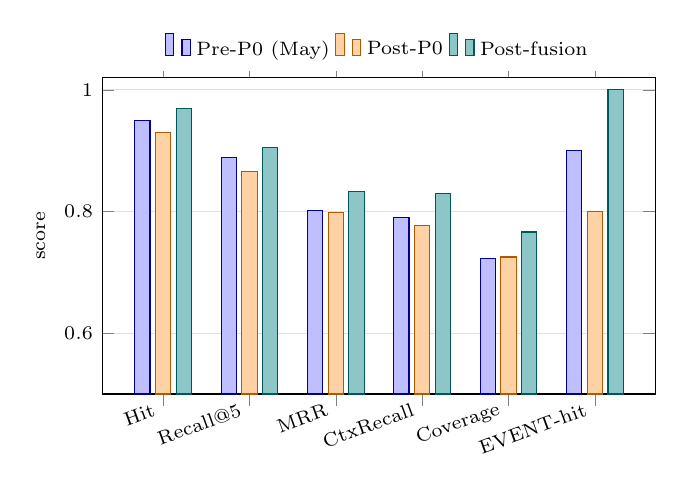
\begin{tikzpicture}
\begin{axis}[
  width=8.6cm, height=5.6cm,
  ybar, bar width=5.5pt,
  enlarge x limits=0.14,
  ymin=0.5, ymax=1.02,
  ylabel={score},
  symbolic x coords={Hit,Recall@5,MRR,CtxRecall,Coverage,EVENT-hit},
  xtick=data,
  x tick label style={font=\scriptsize, rotate=20, anchor=east},
  y tick label style={font=\scriptsize},
  ylabel style={font=\scriptsize},
  legend style={font=\scriptsize, at={(0.5,1.02)}, anchor=south,
                legend columns=3, draw=none},
  ymajorgrids, grid style={black!12},
]
\addplot+[fill=blue!25, draw=blue!60!black] coordinates
  {(Hit,0.950) (Recall@5,0.8892) (MRR,0.8020) (CtxRecall,0.7908)
   (Coverage,0.7223) (EVENT-hit,0.90)};
\addplot+[fill=orange!35, draw=orange!70!black] coordinates
  {(Hit,0.930) (Recall@5,0.8658) (MRR,0.7978) (CtxRecall,0.7767)
   (Coverage,0.7253) (EVENT-hit,0.80)};
\addplot+[fill=teal!45, draw=teal!70!black] coordinates
  {(Hit,0.970) (Recall@5,0.9058) (MRR,0.8335) (CtxRecall,0.8297)
   (Coverage,0.7664) (EVENT-hit,1.00)};
\legend{Pre-P0 (May), Post-P0, Post-fusion}
\end{axis}
\end{tikzpicture}
\caption{The three-round shape of the evidence chain: the KG
completeness overhaul alone (orange) reads flat-to-negative on a
head-entity benchmark; unlocking the ranking layer (teal) recovers and
surpasses every indicator.}
\label{fig:evolution}
\end{figure}

Table~\ref{tab:evolution} and Fig.~\ref{fig:evolution} give the
headline: hit rate 0.97, recall@5 0.906, context recall 0.830, coverage
0.766; EVENT hit rate 1.00 with context recall 0.728 --- not merely
recovering the P0 regression but surpassing the pre-P0 state on every
EVENT indicator; and the margin over the semantic baseline widened to
$+0.16$ hit rate / $+0.148$ recall@5. Four questions flipped
from miss to hit --- the two persistent pre-P0 failures (EVENT\_008 via
aliases$+$EQ, EVENT\_014 via curated node $+$ fusion) and the two TSK
casualties (EVENT\_017 via TSK declassing, EVENT\_019 via the
keyword-exact pin) --- and all five forensic cases of
Table~\ref{tab:tskforensic} recovered, with EVENT\_015 regaining full
recall (its Matthew and Luke anchors returned to the top-5). The quick retrieval loop and
the full pipeline agree bit-exactly on every retrieval metric.

Two residuals are instructive rather than problematic. GENERAL NDCG sits
$0.08$ below post-P0 --- traced per question to the \emph{retirement} of
pin-based artificial top-1 placement (the correct passages remain in
top-5; the earlier perfect MRR was pin manufactured, so the ``drop'' is
the removal of an artifact, not a regression). PERSON\_004 remains the
single PERSON miss, by design out of scope for ranking repairs
(Section~\ref{sec:diagnosis}).

\subsection{$\alpha$ Ablation: A Complementary Structure}
\label{sec:ablation}

Sweeping the fusion coefficient with everything else fixed
(Table~\ref{tab:ablation}) decomposes the remediation:

\begin{table}[!t]
\caption{$\alpha$ Ablation (Retrieval-Only Loop; All Other Repairs
Active)}
\label{tab:ablation}
\centering
\begin{threeparttable}
\begin{tabular}{@{}lcc@{}}
\toprule
 & $\alpha=0$ (pure reranker) & $\alpha=0.3$ (deployed) \\
\midrule
Overall hit rate & 0.97 & 0.97 \\
EVENT hit rate & 1.00 & 1.00 \\
EVENT recall@5 & baseline & $+0.025$ \\
TOPIC MRR & baseline & $+0.133$ \\
NDCG@5 & baseline & $-0.02$ \\
\bottomrule
\end{tabular}
\begin{tablenotes}\footnotesize
\item $\alpha=0$ keeps the data repairs, chunk remap, pin changes, and
keyword-exact pin; only the fusion term is disabled.
\end{tablenotes}
\end{threeparttable}
\end{table}

\begin{itemize}
\item \textbf{Discrete repairs saturate hit rate.} At $\alpha=0$, hit
rate is already 0.97 and EVENT already 1.00: curated data (aliases,
nodes) and the dictionary pin are responsible for \emph{whether} the
answer appears at all.
\item \textbf{Continuous fusion recovers the tail.} $\alpha=0.3$ adds
EVENT recall@5 $+0.025$ --- the multi-gospel parallel anchors of the
Last Supper carry $s_{\mathrm{rr}}\approx 0.01$--$0.02$ and only fusion
returns them --- and TOPIC MRR $+0.133$, at the cost of NDCG@5
$-0.02$ (high-prior, low-surface-form candidates advancing).
\item \textbf{The trade resolves by downstream use.} All top-5 passages
enter the generation context, so recall dominates internal ordering;
$\alpha=0.3$ was adopted.
\end{itemize}

The two mechanisms substitute for the reranker's surface-form monopoly
at \emph{different layers} --- discrete repairs at the
candidate/vocabulary layer, fusion at the scoring layer --- and their
effects are complementary rather than redundant. This
decomposition is the constructive counterpart of the negative result:
the same graph assets that read as zero in Section~\ref{sec:p0} produce
the Table~\ref{tab:evolution} gains once the ranking layer transmits
them.

%% ============================================================================
%% Sections XI-XIV: Discussion, Limitations, Future Work, Conclusion
%% ============================================================================

\section{Discussion}
\label{sec:discussion}

\subsection{Three Co-Determinants of Observable Benefit}

The central methodological claim of this paper is that in a GraphRAG
system, \textbf{knowledge-graph construction quality, the retrieval
ranking mechanism, and benchmark design jointly determine observable
benefit} --- and any one of the three can silently zero out investment
in the others. The evidence chain is summarized by the paper's
three-round structure: a completeness overhaul whose construction
metrics all moved (anchor coverage $+14.4$\,pt, event completeness
$+50$\,pt, cross-references $\times 273$) read as \emph{zero} through a
reranker-monopolized ranking onto a head-saturated benchmark
(Section~\ref{sec:p0}); one day of ranking-layer repair then released
more measured value than the week-scale re-extraction program was
projected to deliver on the same benchmark (Section~\ref{sec:fusion}).
The practical rule we draw: \emph{optimization order should follow the
bottleneck layer, not the upstream-first order of the data flow} ---
and the bottleneck is found by per-question forensics, not by metric
staring.

\subsection{Three Independent Rounds of the Same Lesson}

\begin{table}[!t]
\caption{Three Incidents, One Mechanism: Graph Assets Gated by
Retrieval-Side Machinery}
\label{tab:threerounds}
\centering
\begin{threeparttable}
\footnotesize
\begin{tabular}{@{}p{1.35cm}p{2.5cm}p{2.1cm}p{1.55cm}@{}}
\toprule
Round & Asset in the graph & Gating mechanism & Resolution \\
\midrule
May 2026 & entity vectors (EQ) bridging modern phrasing & reranker
surface-form monopoly & EQ disabled; re-enabled under fusion \\
P0 (July) & correct anchors newly in pool; TSK breadth & same monopoly
$+$ vote-ranked topical noise & fusion $+$ provenance-stratified
weights \\
Dual-anchor family & \emph{all} needed cross-book edges present &
1-hop expansion depends on seed correctness & open (query
decomposition) \\
\bottomrule
\end{tabular}
\end{threeparttable}
\end{table}

Table~\ref{tab:threerounds} aligns the three incidents. The third
deserves elaboration because it was discovered \emph{after} the fusion
remediation and is therefore an independent probe. The two remaining
GENERAL misses are one family: cross-book
\emph{prophecy--fulfillment} questions requiring two anchor sets
simultaneously (GENERAL\_006: Jeremiah's new covenant in Hebrews, gold
$=$ Jer.~31:31--34 $+$ Heb.~8; GENERAL\_008: Zechariah's prophecies in
Passion Week, gold $=$ Zech.~9:9; 11:12--13; 12:10 $+$ Matt.~21/27).
Live graph verification shows \textbf{every needed cross-reference edge
exists} --- Jer.~31$\leftrightarrow$Heb.~8 (3 edges),
Zech.~9$\leftrightarrow$Matt.~21 (2), Zech.~11$\leftrightarrow$Matt.~27
(5), Zech.~12$\leftrightarrow$John~19 (2); TSK is \emph{designed} for
exactly this relation. The failure is upstream of ranking: retrieval
seeds land in the wrong chapters (``prophecy'' surface forms hit the
false-prophet conflict of Jer.~26/28/29; ``Zechariah'' hits the
Zerubbabel visions of Zech.~4), and 1-hop expansion from wrong seeds
cannot reach right edges. Assets in the graph; value gated by the
seed-selection mechanism. These two questions also post the two
lowest answer-correctness scores of the entire suite ($\approx 0.13$,
stable across re-judged runs).

\subsection{Retrieval-to-Answer Attenuation}

Post-fusion, retrieval improved sharply (context recall $+0.053$) while
answer correctness moved $+0.021$ --- at the edge of judge noise. A
clean single-question case isolates the attenuation: EVENT\_005
achieves perfect retrieval (context recall $1.0$, recall@5 $1.0$) yet
its judged answer scores only $0.4$ coverage and $0.173$ correctness on
the run of record --- and re-judging the identical outputs moves those
to $0.70$/$0.353$, an instability that is itself the judge noise of
Section~\ref{sec:evalmetrics} at work. Faithfulness is flat across all
three time points ($\approx 0.95$), so the gains genuinely come from
better context; the loss occurs in the small generation model
(Gemma~4 E4B) and in the judged metrics themselves. The pipeline's
quality bottleneck has, for these questions, \emph{moved past
retrieval} --- consistent with our framing that the observable-benefit
chain must be examined end to end. Any answer-model A/B here must first
neutralize the noncommittal-refusal artifact of
Section~\ref{sec:evalmetrics}, or the honest model loses by
construction --- the local instance of the evaluation-bias warnings
in~\cite{zeng2025unbiased}.

\subsection{Benchmark Saturation: Evaluation Design as Prerequisite}

At 97/100 (VERSE, TOPIC, EVENT at 1.00 hit rate), the benchmark is
saturated in the head, and the three residual misses belong to two
families that need \emph{new architecture}, not better ranking:
cross-chapter aggregation (PERSON\_004; the community-summary/RAPTOR
layer~\cite{edge2024graphrag,sarthi2024raptor}) and cross-book
dual-anchor conjunction (GENERAL\_006/008; query decomposition).
Consequently, \emph{every} remaining roadmap item --- long-tail
re-extraction (P1), event-temporal modeling
(P2,~\cite{lairgi2025atom,zhang2025entityevent,sun2025dygrag}),
hierarchical aggregation (P3) --- would read as zero on this yardstick:
P1's tail improvements are unread by head questions (proved empirically
by P0), P2's target questions already retrieve perfectly (their loss is
in the attenuation chain above), and P3's target population is $n=1$.
The methodological consequence: \textbf{benchmark redesign is the
prerequisite for all further optimization}, not a reporting
afterthought. We specify the needed instruments in
Section~\ref{sec:future}; the general principle --- that the benchmark
itself gates which layer's investment is visible --- echoes the
defect-sensitivity methodology of BRINK~\cite{zhou2025brink} and the
task-dependence findings of~\cite{xiang2025whengraphs}. A cautionary
corollary from Section~\ref{sec:fusion}: with $n=2$ family sizes, tuning
the system on the residual misses would be overfitting; the family must
be \emph{populated first}, then fixed.

\subsection{Patch Lifecycles Under Architecture Evolution}

The pin audit (Section~\ref{sec:fusionlayer}) generalizes: the EQ pin
and graph-uncertainty pin were correct \emph{for the architecture they
were built in} --- discrete rescues under a ranking that discarded
graph signal. Once fusion transmitted that signal continuously, the
same pins became net-negative (noise promotion), and the ``regression''
observed when retiring them (GENERAL NDCG $-0.08$) was itself an
artifact of the artificial placements they used to manufacture.
Remediation machinery must be re-audited whenever the layer it
compensates for changes; yesterday's fix is today's bug. We suspect
this lifecycle is common in deployed RAG systems, where discrete
patches accrete around ranking layers precisely because ranking is the
last mile.

\subsection{Cost and Privacy}

All conclusions above were reached with every model local --- embedder,
reranker, extraction classifiers, generator, and judge --- on a single
GPU host. Round 0 established that a locally served 8-bit E4B-class
model matches a commercial API model end to end on this task within
4\,pp on six of seven metrics~(Table~\ref{tab:round0}); nothing in the
later rounds required revisiting that conclusion, because all
optimization value was retrieval-side. For sensitive religious-domain
deployments --- where both the corpus and user questions may be
confidential --- this is the operative cost/privacy result: the
investment frontier is retrieval and evaluation engineering, not model
procurement.

\section{Limitations}
\label{sec:limitations}

\textbf{Knowledge-graph residuals.} 164 chunk-only entities still lack
pericope-level \textsc{mentions} in the graph itself (retrieval-side
remap restores their visibility, the graph remains incomplete); alias
coverage is $\sim$0.8\% of entities (dictionary and curated sources are
exhausted; mass production requires entity-resolution merge-back);
67{,}306 relation candidates remain unclassified (the 77{,}953-pair
pile minus the 10{,}647 Event-related pairs consumed or set aside by
the P0 rescue); the event layer has
only 26 native temporal/causal Event--Event edges live (the audit-time
figure of 45 included miscounted person-succession edges and edges of
since-deleted generic events) plus 277 unrescued Event--Event
candidates; there is no coreference resolution; toneless-pinyin IDs can
over-merge homophones; and duplicate-name splits (\eg Israel as
Place vs.\ Israelites as Group) await entity resolution.

\textbf{Benchmark scale and head bias.} 100 questions, 20 per category,
asking predominantly head entities; per-category deltas below
$\approx 0.05$ on judged metrics are noise, and several architectural
claims rest on question families of size 1--2, which we deliberately
refuse to tune against.

\textbf{Judged metrics.} RAGAS scores carry $\pm 0.4$ per-question
noise at our scale and a noncommittal rule that penalizes honest
refusal; the answer-coverage judge is a single local model. All
retrieval claims are therefore anchored to deterministic metrics.

\textbf{Generation.} The deployed generator is an 8-bit E4B-class
model; the attenuation analysis shows it discards part of the retrieval
gains. Conclusions about answer quality are conservative lower bounds.

\textbf{Scope.} One corpus, one language, one translation, one domain.
The architecture's signal set and dictionaries are domain-engineered;
transfer requires re-instantiating those assets (though the
methodological findings --- ranking-layer gating, benchmark dependence,
patch lifecycles --- are domain-agnostic claims about system structure,
not about the Bible).

\section{Future Work}
\label{sec:future}

\textbf{Evaluation first.} Per Section~\ref{sec:discussion}, the next
artifact is the benchmark, not the pipeline: (i) long-tail question
sets targeting chunk-only entities and split-pericope person$\times$event
material; (ii) BRINK-style defect injection~\cite{zhou2025brink} ---
remove known edges, measure answer degradation --- as a causal probe of
KG value that no head benchmark can fake; (iii) population of the
cross-chapter-aggregation and dual-anchor families to statistically
meaningful sizes; (iv) judged-metric hygiene (noncommittal exclusion,
position/length debiasing~\cite{zeng2025unbiased}).

\textbf{P1 --- decoupled re-extraction.} Feed extraction whole
pericopes (storage unit $\ne$ extraction unit~\cite{neo4jbuilder});
add a coreference pass scoped to pericope$+$chapter context following
the LINK-KG recipe~\cite{meher2025linkkg}; adopt true-loop gleanings as
in the GraphRAG lineage~\cite{edge2024graphrag} (\eg the nano-graphrag
implementation~\cite{nanographrag}); post-hoc entity resolution with
lexical$+$embedding double signals and propose-then-confirm merging,
writing merged surface forms back as aliases (the alias-generation
mechanism identified in the cross-system survey); type assignment by
majority vote; description regeneration by merge-and-summarize
(cf.~LightRAG~\cite{guo2024lightrag}); ontology-grounded
post-correction as the cheap alternative to
re-extraction~\cite{loconte2026betterlater,zhang2024edc}; and KG
denoising with downstream verification~\cite{zheng2025lessismore}.

\textbf{P2 --- the event-temporal layer.} Promote the event layer from
participants/places (now 84\%/75.5\%) to temporal--causal structure,
following atomic-fact dual-time construction~\cite{lairgi2025atom} and
entity--event dual-graph designs~\cite{zhang2025entityevent,sun2025dygrag};
the 77{,}953-pair provenance-kept rejection pile and the 277 unrescued
Event--Event candidates are the ready inputs.

\textbf{P3 --- aggregation retrieval.} Community summaries (Leiden
partitions~\cite{traag2019leiden} as in~\cite{edge2024graphrag}) or
RAPTOR-style summary trees~\cite{sarthi2024raptor} for
cross-chapter aggregation; RAKG-style pre-entity
re-retrieval~\cite{zhang2025rakg} and cross-chunk graph
augmentation~\cite{zhang2026crossaug} for cross-boundary relations.

\textbf{Retrieval mechanics.} Query decomposition for dual-anchor
conjunctions (retrieve prophecy and fulfillment sides separately, then
join on cross-reference edges); theme-level anchoring; and, if the
strategy-prior fusion reaches its ceiling, calibrated score fusion in
the spirit of~\cite{bacellar2026calibrated} or graph-native retrieval
scoring~\cite{gutierrez2025hipporag2,wang2025archrag}.

\textbf{Generation.} Answer-model A/B under debiased judging, since the
attenuation analysis locates the next bottleneck there.

\section{Conclusion}
\label{sec:conclusion}

We presented the complete architecture of a deployed GraphRAG system
for Traditional Chinese Bible QA --- from layout-geometric PDF parsing,
pericope-centric chunking, grounded dual-track entity extraction,
closed-schema relation extraction, and a three-source cross-reference
network, through a signal-adaptive six-route retrieval design
terminated by cross-encoder reranking and linear rank fusion --- and an
unusually complete empirical record of optimizing it: a quantified
audit tracing KG damage to granularity inheritance rather than chunk
parameters; a completeness overhaul whose construction metrics all
moved and whose benchmark reading was zero; the question-level
diagnosis of that negative result; and a one-day ranking-layer
remediation that surpassed all prior results (hit rate 0.97, EVENT
1.00, $+0.16$ over the semantic baseline), decomposed by ablation into
complementary discrete and continuous mechanisms.

The system-level conclusions are, we believe, portable to any GraphRAG
deployment. Graph assets have no value until the ranking layer
transmits them; benchmark design decides which layer's investment is
visible at all; discrete patches have architecture-bound lifetimes; and
the correct optimization order follows the measured bottleneck, not the
data flow. In our deployment, honoring these rules delivered, in a
day of work, a larger measured return than the deferred week-scale
re-extraction plan was projected to yield on the same benchmark --- and
identified the next bottlenecks (benchmark design, then generation)
before any further construction spend.

%% ============================================================================
%% Appendices
%% ============================================================================

\appendices

\section{Stage-to-Citation Map}
\label{app:citations}

Table~\ref{tab:citemap} indexes, for every pipeline stage and
experimental round, the literature it draws on and the role each work
plays --- so that each citation can be audited in place.

\begin{table*}[!t]
\caption{Which Work Is Cited at Which Stage, and Why}
\label{tab:citemap}
\centering
\begin{threeparttable}
\begin{tabular}{@{}p{3.5cm}p{4.1cm}p{9.2cm}@{}}
\toprule
Stage (section) & Works & Role of the citation \\
\midrule
Problem framing (\S\ref{sec:intro}) &
\cite{hilliard2025flourishing,lewis2020rag,gao2023ragsurvey,edge2024graphrag,peng2026graphragsurvey} &
faith-dimension LLM deficits motivating grounded QA; RAG foundations and
surveys; GraphRAG paradigm \\
\addlinespace
Chunking \& granularity (\S\ref{sec:chunking}, \S\ref{sec:audit} M5--M6) &
\cite{chen2024bgem3,edge2024graphrag,lairgi2025atom,liu2024lost} &
tokenizer/embedder fit; chunk size $\to$ extraction density (600 vs.\
2{,}400 tokens $\approx 2\times$ entity references); finer units extract
more completely; long-context degradation as the upper bound \\
\addlinespace
Coreference \& overlap (\S\ref{sec:audit} M4) &
\cite{yao2019docred} &
40.7\% of relational facts cross-sentence, 17.6\% need coreference ---
the structural ceiling of fragment-local extraction without coreference
(used as \emph{indirect} evidence; no peer-reviewed overlap-size
quantification exists) \\
\addlinespace
Entity extraction (\S\ref{sec:entity}) &
\cite{ckip,gemmateam2025gemma3,meher2025corekg,meher2025insidecorekg} &
Chinese segmentation/NER; the local classify-only LLM; structured
prompting as noise suppression \\
\addlinespace
Relation extraction (\S\ref{sec:relation}) &
\cite{bian2025kgsurvey,huang2025tcrqf} &
schema-based paradigm positioning; evidence-span grounding against
context-divorced triples \\
\addlinespace
Cross-references / TSK (\S\ref{sec:crossrefs}) &
\cite{tsk,zheng2025lessismore} &
public-domain cross-reference data; repair-by-reweighting rather than
deletion \\
\addlinespace
KG-quality remediation roadmap (\S\ref{sec:audit}, \S\ref{sec:future}) &
\cite{meher2025linkkg,zhang2024edc,loconte2026betterlater,zhang2025rakg,zhang2026crossaug,neo4jbuilder,nanographrag,guo2024lightrag} &
coreference recipe ($-45\%$ duplication, length-amplified); post-hoc
canonicalization / correction; cross-chunk reassembly; storage
$\ne$ extraction unit; true-loop gleanings; merge-and-summarize
descriptions \\
\addlinespace
Retrieval substrate (\S\ref{sec:strategies}) &
\cite{karpukhin2020dpr,robertson2009bm25,cormack2009rrf,chen2024bgem3} &
dense retrieval; BM25; RRF hybrid; embedder and cross-encoder \\
\addlinespace
Rank fusion (\S\ref{sec:fusionlayer}, \S\ref{sec:ablation}) &
\cite{bacellar2026calibrated} &
calibrated graph/vector fusion as the sophisticated alternative to our
single-$\alpha$ linear form \\
\addlinespace
Evaluation framework (\S\ref{sec:eval}) &
\cite{es2023ragas,zeng2025unbiased} &
RAGAS metrics; judge-bias methodology (position/verbosity;
noncommittal artifact) \\
\addlinespace
Negative result \& benchmark dependence (\S\ref{sec:p0},
\S\ref{sec:discussion}) &
\cite{zhou2025brink,zeng2025unbiased,xiang2025whengraphs} &
KG-defect $\to$ answer non-linearity and defect injection; debiased
gains; when graphs help RAG at all \\
\addlinespace
Aggregation \& event layer (future) (\S\ref{sec:diagnosis},
\S\ref{sec:future}) &
\cite{sarthi2024raptor,edge2024graphrag,traag2019leiden,lairgi2025atom,zhang2025entityevent,sun2025dygrag,gutierrez2025hipporag2,wang2025archrag} &
RAPTOR trees / Leiden community summaries for cross-chapter
aggregation; temporal--causal event modeling; graph-native retrieval
scoring \\
\addlinespace
Retrieval-side chunking sensitivity (\S\ref{sec:related}) &
\cite{shaukat2026chunking} &
cited \emph{only} for retrieval-downstream chunking sensitivity ---
explicitly not extrapolated to KG construction \\
\bottomrule
\end{tabular}
\end{threeparttable}
\end{table*}

\section{Reproducibility Notes}
\label{app:repro}

\textbf{Determinism and re-scoring.} All retrieval metrics are computed
programmatically against pericope-level gold references; every
evaluation run archives per-question raw responses (sources,
strategies, raw reranker and fused scores, route), and the metric suite
can be recomputed bit-exactly from the archives. The fast
retrieval-only loop was validated to agree bit-exactly with the full
pipeline on all retrieval metrics.

\textbf{Comparability across the three time points.} Answer model
(Gemma~4 E4B, 8-bit), judge model (Gemma~4 26B), decoding temperature
(0.1), top-$k$ (5), and route distribution (R1$=$20, R2$=$25, R3$=$21,
R4$=$18, R5$=$10, R6$=$4, fallback$=$2) were verified identical; the
entity-query strategy was off at the first two time points and on after
the fusion round (its re-enablement is itself one of the audited
repairs). The only other systematic difference between time points is
the state of the knowledge graph and of the post-retrieval chain, as
described in the text.

\textbf{Rollbackability.} Every P0 and fusion-round mutation is
reversible: backfilled mention edges, co-occurrence relation edges, and
TSK cross-reference edges carry provenance flags and can be deleted by
a single predicate each; curated event nodes carry a source tag;
alias injections have before-snapshots; and the rank-fusion layer,
expansion caps, and entity-query strategy are configuration switches
whose legacy settings reproduce the pre-remediation system exactly.

\textbf{Scale of the evaluation.} A full 100-question pipeline run
takes $\approx 2.5$ hours on the single-host deployment (36 min
collection, 1\,h\,42\,m RAGAS judging, 13 min coverage judging); the
retrieval-only loop takes $\approx 15$ minutes and was used for the
$\alpha$ sweep and regression forensics.


\balance
%% ============================================================================
%% References — manual thebibliography in IEEE style.
%% Ordering: first-citation order (verified by tools/check_cite_order.py).
%% Every arXiv entry was verified against the arXiv API (title + authors)
%% on 2026-07-07; software/online entries verified against their live repos.
%% ============================================================================

\begin{thebibliography}{40}

\bibitem{hilliard2025flourishing}
E.~Hilliard \emph{et al.}, ``Measuring AI alignment with human
flourishing,'' arXiv:2507.07787, 2025.

\bibitem{lewis2020rag}
P.~Lewis \emph{et al.}, ``Retrieval-augmented generation for
knowledge-intensive NLP tasks,'' in \emph{Adv. Neural Inf. Process. Syst.
(NeurIPS)}, vol.~33, 2020.

\bibitem{edge2024graphrag}
D.~Edge \emph{et al.}, ``From local to global: A graph RAG approach to
query-focused summarization,'' arXiv:2404.16130, 2024.

\bibitem{peng2026graphragsurvey}
B.~Peng \emph{et al.}, ``Graph retrieval-augmented generation: A survey,''
\emph{ACM Trans. Inf. Syst.}, vol.~44, no.~2, 2026, doi:
10.1145/3777378.

\bibitem{tsk}
\emph{Treasury of Scripture Knowledge}, public-domain cross-reference
dataset (via OpenBible.info). [Online]. Available:
\url{https://github.com/scrollmapper/bible_databases}

\bibitem{yao2019docred}
Y.~Yao \emph{et al.}, ``DocRED: A large-scale document-level relation
extraction dataset,'' in \emph{Proc. 57th Annu. Meeting Assoc. Comput.
Linguistics (ACL)}, 2019.

\bibitem{meher2025corekg}
D.~Meher, C.~Domeniconi, and G.~Correa-Cabrera, ``CORE-KG: An LLM-driven
knowledge graph construction framework for human smuggling networks,''
arXiv:2506.21607, 2025.

\bibitem{meher2025insidecorekg}
D.~Meher and C.~Domeniconi, ``Inside CORE-KG: Evaluating structured
prompting and coreference resolution for knowledge graphs,''
arXiv:2510.26512, 2025.

\bibitem{meher2025linkkg}
D.~Meher, C.~Domeniconi, and G.~Correa-Cabrera, ``LINK-KG: LLM-driven
coreference-resolved knowledge graphs for human smuggling networks,''
arXiv:2510.26486, 2025.

\bibitem{zhou2025brink}
D.~Zhou \emph{et al.}, ``What breaks knowledge graph based RAG?
Benchmarking and empirical insights into reasoning under incomplete
knowledge,'' arXiv:2508.08344, 2025.

\bibitem{zeng2025unbiased}
Q.~Zeng \emph{et al.}, ``How significant are the real performance gains?
An unbiased evaluation framework for GraphRAG,'' arXiv:2506.06331, 2025.

\bibitem{gao2023ragsurvey}
Y.~Gao \emph{et al.}, ``Retrieval-augmented generation for large language
models: A survey,'' arXiv:2312.10997, 2023.

\bibitem{karpukhin2020dpr}
V.~Karpukhin \emph{et al.}, ``Dense passage retrieval for open-domain
question answering,'' in \emph{Proc. Conf. Empirical Methods Natural
Lang. Process. (EMNLP)}, 2020.

\bibitem{robertson2009bm25}
S.~Robertson and H.~Zaragoza, ``The probabilistic relevance framework:
BM25 and beyond,'' \emph{Found. Trends Inf. Retr.}, vol.~3, no.~4, pp.
333--389, 2009.

\bibitem{cormack2009rrf}
G.~V. Cormack, C.~L.~A. Clarke, and S.~B\"uttcher, ``Reciprocal rank
fusion outperforms Condorcet and individual rank learning methods,'' in
\emph{Proc. 32nd Int. ACM SIGIR Conf.}, 2009, pp. 758--759.

\bibitem{chen2024bgem3}
J.~Chen, S.~Xiao, P.~Zhang, K.~Luo, D.~Lian, and Z.~Liu,
``M3-Embedding: Multi-linguality, multi-functionality,
multi-granularity text embeddings through self-knowledge
distillation,'' in \emph{Findings Assoc. Comput. Linguistics: ACL},
2024.

\bibitem{ckip}
CKIP Lab, ``CKIP Transformers'' [Software], 2020. [Online]. Available:
\url{https://github.com/ckiplab/ckip-transformers}

\bibitem{bacellar2026calibrated}
A.~Bacellar, ``Calibrated fusion for heterogeneous graph-vector retrieval
in multi-hop QA,'' arXiv:2603.28886, 2026.

\bibitem{guo2024lightrag}
Z.~Guo, L.~Xia, Y.~Yu, T.~Ao, and C.~Huang, ``LightRAG: Simple and fast
retrieval-augmented generation,'' arXiv:2410.05779, 2024.

\bibitem{gutierrez2025hipporag2}
B.~J. Guti\'errez, Y.~Shu, W.~Qi, S.~Zhou, and Y.~Su, ``From RAG to
memory: Non-parametric continual learning for large language models,'' in
\emph{Proc. Int. Conf. Mach. Learn. (ICML)}, 2025.

\bibitem{wang2025archrag}
S.~Wang, Y.~Fang, Y.~Zhou, X.~Liu, and Y.~Ma, ``ArchRAG: Attributed
community-based hierarchical retrieval-augmented generation,''
arXiv:2502.09891, 2025.

\bibitem{sarthi2024raptor}
P.~Sarthi, S.~Abdullah, A.~Tuli, S.~Khanna, A.~Goldie, and
C.~D. Manning, ``RAPTOR: Recursive abstractive processing for
tree-organized retrieval,'' in \emph{Proc. Int. Conf. Learn. Represent.
(ICLR)}, 2024.

\bibitem{zhang2025entityevent}
Z.~Y. Zhang, Z.~Li, Y.~Li, B.~Ding, and B.~K.~H. Low, ``Respecting
temporal-causal consistency: Entity-event knowledge graphs for
retrieval-augmented generation,'' arXiv:2506.05939, 2025.

\bibitem{sun2025dygrag}
Q.~Sun \emph{et al.}, ``DyG-RAG: Dynamic graph retrieval-augmented
generation with event-centric reasoning,'' arXiv:2507.13396, 2025.

\bibitem{xiang2025whengraphs}
Z.~Xiang \emph{et al.}, ``When to use graphs in RAG: A comprehensive
analysis for graph retrieval-augmented generation,'' arXiv:2506.05690,
2025.

\bibitem{bian2025kgsurvey}
H.~Bian, ``LLM-empowered knowledge graph construction: A survey,''
arXiv:2510.20345, 2025.

\bibitem{liu2024lost}
N.~F. Liu \emph{et al.}, ``Lost in the middle: How language models use
long contexts,'' \emph{Trans. Assoc. Comput. Linguistics}, vol.~12, pp.
157--173, 2024.

\bibitem{loconte2026betterlater}
L.~Loconte, T.~Hospedales, and C.~Cornelio, ``Better later than sooner:
Neuro-symbolic knowledge graph construction via ontology-grounded
post-extraction correction,'' arXiv:2605.29168, 2026.

\bibitem{zhang2024edc}
B.~Zhang and H.~Soh, ``Extract, define, canonicalize: An LLM-based
framework for knowledge graph construction,'' in \emph{Proc. Conf.
Empirical Methods Natural Lang. Process. (EMNLP)}, 2024.

\bibitem{zheng2025lessismore}
Y.~Zheng \emph{et al.}, ``Less is more: Denoising knowledge graphs for
retrieval augmented generation,'' arXiv:2510.14271, 2025.

\bibitem{zhang2025rakg}
H.~Zhang \emph{et al.}, ``RAKG: Document-level retrieval augmented
knowledge graph construction,'' arXiv:2504.09823, 2025.

\bibitem{huang2025tcrqf}
M.~Huang, C.~Bu, Y.~He, and X.~Wu, ``How to mitigate information loss in
knowledge graphs for GraphRAG: Leveraging triple context restoration and
query-driven feedback,'' arXiv:2501.15378, 2025.

\bibitem{zhang2026crossaug}
J.~Zhang, Y.~Zhao, J.~Yu, J.~Yu, and X.~Li, ``Beyond chunk-local
extraction: Cross-chunk graph augmentation for GraphRAG,''
arXiv:2605.28004, 2026.

\bibitem{lairgi2025atom}
Y.~Lairgi, L.~Moncla, K.~Benabdeslem, R.~Cazabet, and P.~Cl\'eau,
``ATOM: AdapTive and OptiMized dynamic temporal knowledge graph
construction using LLMs,'' in \emph{Findings Assoc. Comput. Linguistics:
EACL}, 2026.

\bibitem{es2023ragas}
S.~Es, J.~James, L.~Espinosa-Anke, and S.~Schockaert, ``RAGAS: Automated
evaluation of retrieval augmented generation,'' arXiv:2309.15217, 2023.

\bibitem{shaukat2026chunking}
M.~A. Shaukat, M.~Adnan, and C.~C.~N. Kuhn, ``A systematic investigation
of document chunking strategies and embedding sensitivity,''
arXiv:2603.06976, 2026.

\bibitem{gemmateam2025gemma3}
Gemma Team, ``Gemma 3 technical report,'' arXiv:2503.19786, 2025.

\bibitem{gemma4}
Gemma Team, ``Gemma 4,'' Google DeepMind, Apr. 2026. [Online]. Available:
\url{https://deepmind.google/models/gemma/gemma-4/}

\bibitem{claudehaiku45}
Anthropic, ``Introducing Claude Haiku 4.5,'' Oct. 2025. [Online].
Available: \url{https://www.anthropic.com/news/claude-haiku-4-5}

\bibitem{neo4jbuilder}
Neo4j Labs, ``LLM Knowledge Graph Builder'' [Software]. [Online].
Available: \url{https://github.com/neo4j-labs/llm-graph-builder}

\bibitem{nanographrag}
``nano-graphrag'' [Software]. [Online]. Available:
\url{https://github.com/gusye1234/nano-graphrag}

\bibitem{traag2019leiden}
V.~A. Traag, L.~Waltman, and N.~J. van Eck, ``From Louvain to Leiden:
Guaranteeing well-connected communities,'' \emph{Sci. Rep.}, vol.~9, no.
5233, 2019.

\end{thebibliography}


\end{document}
